\documentclass[10pt, conference]{IEEEtran}
\IEEEoverridecommandlockouts
% The preceding line is only needed to identify funding in the first footnote. If that is unneeded, please comment it out.
\usepackage{cite}
\usepackage{amsmath,amssymb,amsfonts}
\usepackage{algorithmic}
\usepackage{graphicx}
\usepackage{textcomp}
\usepackage{xcolor}
\usepackage{url}
\usepackage{float}
\usepackage{algorithm}
\usepackage{algpseudocode}
\newcommand{\cmark}{\textcolor{green!60!black}{\checkmark}}
\newcommand{\xmark}{\textcolor{red}{\texttimes}}
\usepackage{booktabs}
\usepackage{caption,cuted,booktabs,tabularx,ragged2e,array}
\newcolumntype{Y}{>{\RaggedRight\arraybackslash}X}

\usepackage[most]{tcolorbox}

\def\BibTeX{{\rm B\kern-.05em{\sc i\kern-.025em b}\kern-.08em
    T\kern-.1667em\lower.7ex\hbox{E}\kern-.125emX}}
% ============================================================
\begin{document}
 
\title{From Detection to Action: Blockchain-Governed Agentic AI for Autonomous Network Defense}
 
\author
 {\IEEEauthorblockN{1\textsuperscript{st} MD Shariful Islam}
 \IEEEauthorblockA{\textit{Dept. of Computer Science} \\
 \textit{University of Northern British Columbia}\\
 Prince George, British Columbia \\
 islam5@unbc.ca}
 
 \and
 \IEEEauthorblockN{2\textsuperscript{nd} Sajal Saha}
 \IEEEauthorblockA{\textit{Dept. of Computer Science} \\
 \textit{University of Northern British Columbia}\\
 Prince George, British Columbia \\
 sajal.saha@unbc.ca}

 }
 
\maketitle

\begin{abstract}
Agentic AI can automate network defense, but allowing AI agents to modify live enterprise networks introduces a critical trust problem: generated actions may be incorrect, altered, or inconsistent with security policy. We propose a unified end-to-end architecture that integrates intrusion detection, explainable attribution, policy-grounded mitigation generation, and blockchain-based action enforcement across distributed enterprise network domains. Vertical Federated Learning enables Access, Perimeter, and Endpoint domains to collaboratively detect attacks without sharing raw features, preserving data locality while maintaining performance comparable to centralized learning. SHAP identifies the domain contribution to each alert and guides a retrieval-augmented generation pipeline grounded in ten authoritative cybersecurity frameworks to produce domain-specific mitigation plans.Before execution, security actions are validated against a blockchain-stored whitelist derived from industry standards and established cybersecurity knowledge. Each generated action is deterministically checked against the detected attack type and the corresponding authorized action policy. Only actions that satisfy both checks are released for execution, while their outcomes are recorded on-chain to provide immutable and auditable enforcement. This design separates probabilistic AI reasoning from deterministic enforcement, preventing unapproved or modified actions from reaching the network even when the generated plan is unreliable or has been tampered with. The resulting architecture provides an accountable detection-to-action pipeline in which blockchain serves as the trust and enforcement layer for autonomous network defense.
\end{abstract}

 
\begin{IEEEkeywords}
Vertical Federated Learning,
Agentic AI,
Large Language Models,
Retrieval-Augmented Generation,
Blockchain Trust Enforcement,
Enterprise Network Intrusion Detection,
Smart Contracts,
Distributed Network Security
\end{IEEEkeywords}
 

% ============================================================

\section{Introduction}

The rapid growth of distributed enterprise networks, cloud services, edge devices, and heterogeneous computing environments has significantly increased the complexity of cybersecurity. Modern network attacks can span multiple domains and generate diverse observations across network, perimeter, and endpoint layers, making effective intrusion detection increasingly dependent on combining complementary security information. However, raw security telemetry is often distributed across organizational boundaries and cannot be freely shared because of privacy, data ownership, regulatory, and security constraints~\cite{sharafaldin2018,nist80053,nist800207}.

Artificial intelligence (AI) and machine learning (ML) have become important for identifying complex attack patterns and supporting automated security analysis. Federated Learning (FL) enables collaborative model training without requiring direct exchange of raw data, while Vertical Federated Learning (VFL) is particularly suitable when different parties hold complementary features of the same security events~\cite{liu2024vfl,folino2024}. However, distributed detection alone provides limited insight into why an event is classified as malicious and does not directly determine how the detected threat should be addressed. Explainable attribution is therefore important for identifying the evidence contributing to a detection decision and supporting trustworthy downstream security reasoning.

Recent advances in Large Language Models (LLMs), Retrieval-Augmented Generation (RAG), and Agentic AI provide opportunities to extend cybersecurity systems from detection toward contextual reasoning and autonomous response. LLMs can interpret complex security events, RAG can ground reasoning in external security knowledge, and Agentic AI can plan and execute security actions~\cite{xi2023,li2025,shajarian2026,fu2026}. Security decisions can further be grounded in established frameworks such as MITRE ATT\&CK~\cite{mitre_attack} and NIST SP 800-53~\cite{nist80053}. However, allowing agents to directly execute security actions introduces additional risks, including incorrect reasoning, prompt manipulation, compromised agents, and unauthorized actions.

This creates a fundamental trust requirement between autonomous reasoning and security execution. Blockchain and smart contracts can provide a tamper-resistant and independently verifiable governance layer for agent coordination, authorization, provenance, and policy enforcement~\cite{karim2025,chen2024,jin2024,jan2025}. Nevertheless, existing approaches do not jointly connect privacy-preserving intrusion detection and explainable attribution with grounded mitigation planning and verifiable security-action execution. In particular, an autonomous security system should ensure that an action is not only permitted by policy, but also corresponds to the mitigation plan authorized for the specific detected attack.

Motivated by these challenges, we propose a unified framework that integrates VFL-based intrusion detection, feature-level attribution, RAG-grounded LLM reasoning, Agentic AI planning, and blockchain-governed security enforcement to enable privacy-preserving collaborative intrusion detection and trusted autonomous response. The main contributions of this work are as follows:
\begin{itemize}
  \item A unified end-to-end architecture from detection to mitigation for multi-domain enterprise intrusion response, in which VFL,  SHAP-conditioned RAG, and blockchain enforcement are coupled rather than stacked as optional modules.
  \item Empirical evidence that a three-party VFL detector can approach centralized accuracy on CIC-style traffic while keeping Access, Perimeter, and Endpoint features local.
  \item An apply-time enforcement evaluation in which unauthorized actions and in-cycle plan substitutions are rejected, and accepted actions leave an on-chain audit record.
\end{itemize}

% ============================================================
\section{Related Work}
\label{sec:related}
The use of artificial intelligence (AI) and machine learning (ML) in cybersecurity has gained increasing interest due to their ability to identify complex attack patterns and adapt to evolving threats. This section reviews the literature across four key areas: federated learning for collaborative security, LLM- and RAG-based cybersecurity reasoning, blockchain-based trust and security enforcement, and agentic AI for autonomous security operations. Recent studies have explored these technologies for privacy-preserving detection, knowledge-grounded security reasoning, trusted coordination, and autonomous threat response, while also highlighting challenges related to explainability, governance, and the safe execution of autonomous actions. The review further identifies limitations and research gaps that motivate the proposed framework.

\subsection{Federated Learning in Cybersecurity}
Federated learning (FL) supports collaborative intrusion detection without sharing raw telemetry, and vertical FL (VFL) is used when parties hold complementary features of the same events. Liu \textit{et al.}~\cite{liu2024vfl} map VFL across effectiveness, efficiency, and privacy, and introduce VFLow to balance communication, computation, privacy, effectiveness, and fairness. Folino \textit{et al.}~\cite{folino2024} propose a scalable VFL framework for privacy-preserving cybersecurity analytics, but without feature-level attribution, which limits interpretability for downstream LLM reasoning and automated response.
 
Alazab \emph{et al.}~\cite{alazab2022}
present the first comprehensive survey on federated learning for cybersecurity, systematically categorizing its applications across authentication, privacy preservation, trust management, and attack detection alongside real-world deployment cases and open research challenges.  Talpini et al.~\cite{talpini2025} proposed the SHIELDED architecture, a distributed federated learning framework integrating network-aware orchestration and SHAP-based anomaly detection, achieving 99.05\% accuracy; however, it lacks LLM/RAG-grounded reasoning and automated security enforcement, limiting its capability for evidence-driven and adaptive response. Amin et al.~\cite{amin2025efficient} proposed an XGBoost--LightGBM FL framework for SDN threat detection and adaptive mitigation, achieving 96.3\% accuracy; however, its conventional FL design does not address heterogeneous feature ownership or provide feature-level attribution and LLM/RAG-grounded reasoning. Yu, Han \textit{et al.}~\cite{yu2024vflprivacy} taxonomize VFL privacy threats and defenses by life-cycle stage, while Ye \textit{et al.}~\cite{ye2024vfl} survey VFL from effectiveness, security, and applicability. Neither connects VFL detection to grounded mitigation or pre-execution action enforcement.

Overall, existing studies establish the effectiveness of FL and VFL for privacy-preserving cybersecurity analytics, but they largely lack integrated feature-level explainability, grounded LLM reasoning, and trustworthy automated security enforcement, motivating a unified framework that connects detection, attribution, reasoning, and response.

\subsection{LLM- and RAG-Based Cybersecurity Reasoning}

Agentic AI has emerged as a promising approach to cybersecurity by enabling autonomous threat detection, decision-making, and incident response. Large Language Model (LLM)-based agents extend conventional security
analytics by introducing reasoning, planning, memory, and tool
interaction~\cite{xi2023}. Li and Zhu~\cite{li2025} formulate Agentic AI for cyber resilience as a detect--reason--act paradigm.
 Fu et al.~\cite{fu2026} proposed FeRAG, a federated RAG-based LLM framework for privacy-preserving cyber threat detection; however, it lacks feature-level explainability and automated, blockchain-governed security enforcement. Kshetri~\cite{kshetri2025agentic} highlights that increasing autonomy also introduces risks such as adversarial manipulation, loss of human oversight, and expanded attack surfaces, emphasizing the need for effective governance and monitoring.
Alsuwaiket et al.~\cite{alsuwaiket2024} proposed ZeroDay-LLM, combining distributed FL, BERT-based threat reasoning, and DQN-based adaptive response to achieve 97.8\% accuracy and 95.7\% zero-day detection; however, it lacks VFL-based attribution, RAG-grounded reasoning, and blockchain-governed enforcement.
However, increased autonomy also introduces new security risks. Lazer \emph{et al.}~\cite{lazer2026} and Chhabra \emph{et al.}~\cite{chhabra2026} identify threats involving agent integrity, accountability, and cross-domain attack propagation. These concerns become more significant when agents can invoke operational tools, since erroneous reasoning, prompt injection, or compromised
agents can translate directly into consequential actions.


\subsection{Blockchain-Governed Trust and Security Enforcement}

As autonomous AI agents increasingly perform security-sensitive actions, trusted execution becomes essential to prevent unauthorized or unintended responses. Blockchain provides a suitable governance layer through tamper-resistant records, decentralized verification, provenance, and smart-contract-based policy enforcement. Recent studies have therefore explored blockchain for trustworthy multi-agent coordination, agent verification, policy enforcement, and autonomous execution.

Karim et al. ~\cite{karim2025} surveyed AI-agent–blockchain integration, highlighting decentralized reasoning and smart-contract governance while leaving VFL-based detection, RAG-grounded reasoning, XAI, and automated cybersecurity enforcement unaddressed.Pendli~\cite{pendli2025} reviewed blockchain-based security for agentic AI, highlighting its role as a trust and governance layer, but lacking an integrated VFL-based detection, XAI attribution, RAG reasoning, and automated security enforcement framework. Chen et al.~\cite{chen2024} proposed BlockAgents, a blockchain-enabled LLM multi-agent framework using Proof-of-Thought consensus, reducing poisoning degradation but lacking VFL, XAI threat attribution, RAG reasoning, and automated security enforcement. Jin et al.~\cite{jin2024} proposed DeCoAgent, an LLM-based decentralized agent framework using few-shot prompting, RAG, and smart contracts, but lacking VFL-based detection, XAI threat attribution, and automated cybersecurity enforcement. 
Alqithami~\cite{alqithami2026} surveyed agent--blockchain interoperability, proposing intent-based execution and verifiable policy enforcement, but lacking VFL-based detection, XAI threat attribution, RAG-grounded reasoning, and automated cybersecurity enforcement.

Chen et al.~\cite{chen2026agentchain} introduced AgentChain, using PoCQ-based decentralized multi-agent consensus and stake reassignment to improve the trustworthiness of LLM-generated responses, reducing poisoning, backdoor, and jailbreak attack success rates to below 4\%; however, it does not address distributed cyberattack detection or security-action enforcement. Syed et al.~\cite{syed2025agentic} integrated LLM reasoning, reinforcement learning, multi-agent coordination, and blockchain-based auditing for autonomous software supply-chain defense, but does not address VFL-based network intrusion detection, feature-level attribution, or event-specific mitigation-plan integrity.

Wickremasinghe et al.~\cite{wickremasinghe2026state} investigated state verification in asynchronous blockchain-driven Agentic AI systems, focusing on state consistency and Byzantine-resilient verification, but does not address cyberattack detection or security-action authorization. Rahmati Tabrizi et al.~\cite{rahmati2025beaf} proposed BEAF, combining blockchain accountability with policy-as-code for high-assurance autonomous AI; however, its focus is clinical AI rather than network intrusion response. Gao et al.~\cite{gao2025trustagentnet} proposed TrustAgentNet, using consortium blockchain to verify agent identities and skillsets, but it does not address attack-specific mitigation planning or plan integrity. 

Fan \textit{et al.}~\cite{fan2025} proposed SecureVFL, a permissioned-blockchain VFL design that uses replicated secret sharing and Proof of Feature Sharing to protect multi-party training without homomorphic encryption; it does not enforce attack-specific mitigation actions. Singh \textit{et al.}~\cite{singh2025zt} implemented Zero Trust on Ethereum, using smart contracts as the policy engine to enforce MFA, RBAC, and just-in-time access, but without an AI planner or mitigation-to-action binding. Zhang \textit{et al.}~\cite{zhang2024exploit}, Xu~\cite{xu2026}, Ressi \textit{et al.}~\cite{ressi2024}, and Nguyen Thanh \textit{et al.}~\cite{nguyen2024} further investigate blockchain for provenance, governance, trustworthy AI, and autonomous-agent ecosystems. Collectively, these approaches strengthen trust, access control, or training integrity, but they do not provide an integrated cybersecurity detection-to-action mechanism.

\begin{strip}
\centering
\captionof{table}{Comparison of related works on blockchain-governed, VFL-based, and agentic-AI cybersecurity frameworks.}
\label{tab:related-work}
\scriptsize
\setlength{\tabcolsep}{2pt}
\renewcommand{\arraystretch}{1.12}
\begin{tabularx}{\textwidth}{@{}YYYYYYY@{}}
\toprule
\textbf{Paper (Year)} & \textbf{Domain / Application} & \textbf{Core Mechanism} & \textbf{Blockchain Type} & \textbf{Consensus / Protocol} & \textbf{Key Contribution} & \textbf{Main Limitation} \\
\midrule
Shajarian \textit{et al.}~\cite{shajarian2026}, ReGAIN (2026) & Network traffic analysis (ICMP / SYN flood) & RAG with MMR sampling, cross-encoder re-ranking & None & N/A & Citation-grounded, hallucination-resistant explanations & 74--76\% precision on ping flood; API latency limits real-time use \\
Fu \textit{et al.}~\cite{fu2026}, FeRAG (2026) & Cyber threat detection in Internet-of-Energy & Federated learning + RAG with vector DBs and RRF re-ranking & None & FL weighted averaging & FL privacy + RAG grounding; GPT-4o + FeRAG = 0.849 F1 & No blockchain governance; detection only, no enforcement \\
Chen \textit{et al.}~\cite{chen2024}, BlockAgents (2024) & Multi-agent problem-solving and planning & Proof-of-Thought (PoT): stake-based miner designation + debate voting & Abstracted & PoT with multi-metric evaluation prompts & Rewards highest-quality ``thought'' with accounting rights & Accuracy drops if malicious agents dominate miner role \\
Jin \textit{et al.}~\cite{jin2024}, DeCoAgent (2024) & Decentralized agent marketplace & Six LLM modules mapping NL $\rightarrow$ smart-contract calls & Ethereum (Ganache / Remix) & Standard Ethereum & LLM converts NL into contract calls for registration and task assignment & No policy/whitelist enforcement; inconsistent LLM outputs \\
Jan \textit{et al.}~\cite{jan2025}, Blockchain-Monitored Agentic AI (2025) & Agentic AI (healthcare, smart city, inventory) & Perception $\to$ Conceptualization $\to$ Blockchain Governance $\to$ MCP Action & Permissioned (Hyperledger Fabric) & Smart-contract validation (Action Registry, Policy Control, Evaluation) & End-to-end blockchain governance of LangChain agents before MCP execution & No mitigation-to-action binding; no XAI \\
Alqithami~\cite{alqithami2026}, Autonomous Agents on Blockchains (2026) & Agent--blockchain interoperability (DeFi, DAOs, treasury) & SLR of 317 works; 5-part taxonomy; Transaction Intent Schema + Policy Decision Record & Public (Ethereum, L2, ERC-4337) & N/A (survey); policy-gated + MEV-aware execution & Threat model for agent-driven transactions; eval-suite proposal & Position paper; abstractions not implemented or benchmarked \\
Chen \textit{et al.}~\cite{chen2026agentchain}, AgentChain (2026) & Trustworthy multi-agent LLM QA (medical) & Decentralized council with Proof-of-Content-Quality (PoCQ) & Abstracted & PoCQ: VRF council + debate voting + stake incentives & Semantic consensus for stochastic LLMs; game-theoretic proofs & FT $<$50\% malicious; large councils show diminishing returns \\
Wickremasinghe \textit{et al.}~\cite{wickremasinghe2026state}, State-verification async blockchain (2026) & Agentic-AI orchestrators over async blockchains & Timed automaton + BFT gossip + ZKP; disagreement as change-detection signal & Async BFT (HoneyBadgerBFT-style) & Async BFT + timed automaton + ZKP; $f=\lfloor(\omega-1)/3\rfloor$ & Solves 37.3\% agent-state mismatch; ZKP-verified responses & Limited to state consistency; no policy or action-execution governance \\
Rahmati-Tabrizi \textit{et al.}~\cite{rahmati2025beaf}, BEAF (2025) & Clinical AI accountability (EU AI Act) & Stakeholder-Risk Matrix + policy-as-code; ZKP overlay & Permissioned (Fabric + Idemix ZKP) & Raft (EtcdRaft), 2-of-3 endorsement & Maps regulatory liability to stakeholders; sub-250\,ms p95 latency & Not attack-focused; auditor UI/UX only partial \\
Gao \textit{et al.}~\cite{gao2025trustagentnet}, TrustAgentNet (2025) & Agentic AI networking (6G), skillset verification & Chain of Skillset (CoS): skillset chain + training chains & Consortium (Hyperledger Fabric) & Etcdraft/Raft + FedAvg + MSP & Verifiable skillset tags; 3-way security/performance/cost trade-off & More consensus nodes increase latency, CPU, and overhead \\


Fan \textit{et al.}~\cite{fan2025}, SecureVFL (2025) & Privacy-preserving VFL (banking) & Replicated Secret Sharing + novel (4,2)-sharing & Permissioned & PoFS + DPoS committee & Addition-only sharing (no HE); 2-of-4 dropout tolerance; anonymous identities & Three-party base protocol fails if any party drops \\

Singh \textit{et al.}~\cite{singh2025zt}, Blockchain-Enabled ZT for FinTech (2025) & FinTech (insider threats, malware, APTs) & Ethereum contracts for MFA, RBAC, and JIT; blockchain as PE/PEP/policy store & Public / consortium Ethereum & Ethereum PoS + smart-contract policy execution & Immutable access control and tamper-proof audit trails; STRIDE-validated & Higher latency and lower throughput; no AI-agent integration \\
\bottomrule
\end{tabularx}
\end{strip}

Table~\ref{tab:related-work} summarizes representative studies across
these research directions. The comparison considers the Domain, core mechanism,
blockchain type, concensus type, key contributions and limitations of each
approach. This overview highlights that existing research has made
substantial progress in individual components of autonomous cyber defense,
but the components are generally investigated independently or in limited
combinations.

%%%%%
%%Table
%%%%%%%%%

To further distinguish the proposed architecture from existing approaches,
Table~\ref{tab:related_work} compares the capabilities provided by
representative studies. We organize these capabilities into two
complementary groups. The first is the \textit{IDS/Intelligence Capability}, covering intrusion detection, explainability, RAG/LLM-based reasoning, and agentic action. The second is the \textit{Governance and Protection Capability}, covering policy grounding, pre-execution protection, and plan integrity.

\newcolumntype{C}{>{\centering\arraybackslash}X}

\begin{table*}[!t]
\centering
\caption{Capability-based comparison of existing autonomous cyber defense approaches.}
\label{tab:related_work}
\renewcommand{\arraystretch}{1.18}
\setlength{\tabcolsep}{3pt}
\scriptsize
\begin{tabularx}{\textwidth}{@{}>{\raggedright\arraybackslash}p{1.8cm}|CCCC|CCC@{}}
\hline
\multicolumn{1}{c|}{\textbf{Related Work}} &
\multicolumn{4}{c|}{\textbf{IDS / Intelligence Capability}} &
\multicolumn{3}{c}{\textbf{Governance \& Protection Capability}} \\
\cline{2-5}\cline{6-8}
&
\textbf{IDS} &
\textbf{XAI} &
\textbf{RAG/LLM} &
\textbf{Agentic Action} &
\textbf{Policy Grounding} &
\textbf{Pre-Execution Protection} &
\textbf{Plan Integrity} \\
\hline
Folino et al.~\cite{folino2024}
& \cmark & \xmark & \xmark & \xmark
& \xmark & \xmark & \xmark \\
ReGAIN~\cite{shajarian2026}
& \cmark & \xmark & \cmark & \xmark
& \cmark & \xmark & \xmark \\
Fu et al.~\cite{fu2026}
& \cmark & \xmark & \cmark & \xmark
& \cmark & \xmark & \xmark \\
BlockAgents~\cite{chen2024}
& \xmark & \xmark & \cmark & \cmark
& \xmark & \cmark & \xmark \\
DeCoAgent~\cite{jin2024}
& \xmark & \xmark & \cmark & \cmark
& \xmark & \cmark & \xmark \\
Jan et al.~\cite{jan2025}
& \xmark & \xmark & \cmark & \cmark
& \cmark & \cmark & \xmark \\
Alazab et al.~\cite{alazab2022}
& \cmark & \xmark & \xmark & \xmark
& \xmark & \xmark & \xmark \\
Talpini et al.~\cite{talpini2025}
& \cmark & \cmark & \xmark & \xmark
& \xmark & \xmark & \xmark \\
Amin et al.~\cite{amin2025efficient}
& \cmark & \xmark & \xmark & \xmark
& \xmark & \xmark & \xmark \\

Alsuwaiket~\cite{alsuwaiket2024}
& \cmark & \xmark & \cmark & \xmark
& \xmark & \xmark & \xmark \\

Alqithami~\cite{alqithami2026}
& \xmark & \xmark & \cmark & \cmark
& \cmark & \xmark & \xmark \\
AgentChain~\cite{chen2026agentchain}
& \xmark & \xmark & \cmark & \cmark
& \xmark & \cmark & \xmark \\
Syed et al.~\cite{syed2025agentic}
& \xmark & \xmark & \cmark & \cmark
& \xmark & \cmark & \xmark \\
Wickremasinghe et al.~\cite{wickremasinghe2026state}
& \xmark & \xmark & \xmark & \cmark
& \xmark & \cmark & \xmark \\
BEAF~\cite{rahmati2025beaf}
& \xmark & \xmark & \xmark & \cmark
& \cmark & \cmark & \xmark \\
TrustAgentNet~\cite{gao2025trustagentnet}
& \xmark & \xmark & \cmark & \cmark
& \xmark & \cmark & \xmark \\
SecureVFL~\cite{fan2025}
& \cmark & \xmark & \xmark & \xmark
& \xmark & \xmark & \xmark \\
Singh et al.~\cite{singh2025zt}
& \xmark & \xmark & \xmark & \xmark
& \cmark & \cmark & \xmark \\
Wu et al.~\cite{wu2023falcon}
& \xmark & \cmark & \xmark & \xmark
& \xmark & \xmark & \xmark \\

\textbf{Our Work}
& \cmark & \cmark & \cmark & \cmark
& \cmark & \cmark & \cmark \\
\hline
\end{tabularx}
\end{table*}

The comparison shows that existing approaches address important components of autonomous cyber defense, but no representative approach jointly connects privacy-preserving detection and explainability with grounded reasoning and blockchain-governed execution. Federated approaches primarily support collaborative intrusion detection, while RAG/LLM-based systems extend cybersecurity analysis with knowledge-grounded reasoning. Blockchain-based agentic systems, in contrast, focus mainly on coordination, trust, policy enforcement, provenance, or execution assurance. Consequently, the integration of these capabilities for autonomous intrusion response remains insufficiently addressed.

A key challenge is ensuring that an autonomous security action is both authorized and faithful to the mitigation decision generated for the corresponding attack. A policy whitelist can verify that an action is generally permitted, but cannot ensure that a compromised agent has not substituted another permitted action. Conversely, an immutable commitment can verify that a mitigation plan has not been modified, but does not establish whether the executed action is authorized for the detected attack. This work addresses these limitations by jointly verifying action authorization against the detected attack class and binding the executed action to the mitigation plan committed for the corresponding detection event. Blockchain therefore serves as a pre-execution governance layer that provides both policy-based authorization and mitigation-plan integrity for trusted autonomous security enforcement.



% ============================================================
% Section III --- paste into the CCNC manuscript.
% Citations use only keys from the current thebibliography.
% Point \ref{fig:e2e} at the existing end-to-end system diagram (Fig.~1).

%% Threat model is missing
\section{Proposed End-to-End Architecture}
\label{sec:system}

The proposed architecture is designed to connect privacy-preserving intrusion detection with grounded security reasoning and controlled mitigation execution. As illustrated in Fig.~\ref{fig:system_diagram}, the system follows a four-stage workflow: \emph{Detect--Reason--Commit--Apply}. The design separates probabilistic components, including machine learning and language-model reasoning, from deterministic security controls that govern whether a generated action can reach the execution layer. The architecture consists of two main components. First, the threat model defines the adversarial capabilities, security assumptions, and failure modes addressed by the system. Second, the end-to-end system design describes how a network event progresses through detection, reasoning, blockchain governance, and controlled execution. The separation is important because the reasoning layer may generate an incorrect or modified mitigation plan, whereas the execution layer must make authorization decisions independently of the language model.


\subsection{Threat Model}

We consider an autonomous network-defense environment in which security
telemetry is distributed across multiple network domains and an AI agent
is responsible for generating mitigation actions. The adversary is
assumed to be capable of influencing or modifying information after
detection but before execution. In particular, we consider threats that
exploit the gap between probabilistic AI-generated mitigation and the
deterministic requirements of security enforcement.

The considered threats and their corresponding security mechanisms are
summarized in Table~\ref{tab:threat_model}. First, an unreliable or
compromised reasoning component may generate an action that is
inappropriate for the detected attack. Second, prompt or context
manipulation may attempt to influence the generated mitigation plan
through misleading or unauthorized context. Third, unauthorized action
selection occurs when the generated plan contains an action that is not
permitted for the detected attack class. Fourth, plan substitution refers
to replacing an action with another valid action from a different
mitigation cycle. Fifth, payload tampering refers to modification of a
previously generated mitigation plan after it has been committed but
before execution. Sixth, wrong-domain execution occurs when an action is
assigned to a network tier different from the one specified by the
mitigation plan. Finally, replay or duplicate execution refers to the
reuse of an already committed or applied action.


\begin{table}[t]
\centering
\caption{Threat model and security mechanisms.}
\label{tab:threat_model}
\small
\begin{tabular}{p{0.24\linewidth}p{0.30\linewidth}p{0.34\linewidth}}
\hline
\textbf{Threat} & \textbf{Capability} & \textbf{Mitigation} \\
\hline

Compromised reasoning
&
Alter or replace the generated plan
&
RAG grounding, constrained actions, deterministic validation
\\

Context manipulation
&
Inject misleading reasoning context
&
Closed corpus, structured context, constrained output
\\

Unauthorized action
&
Select an action not allowed for the attack
&
Attack-specific on-chain whitelist
\\

Plan substitution
&
Replace an action across mitigation cycles
&
Per-event plan commitment
\\

Payload tampering
&
Modify a committed mitigation plan
&
SHA-256 commitment and re-hashing
\\

Wrong-domain execution
&
Change the assigned network domain
&
Domain/tier consistency check
\\

Replay / duplicate execution
&
Reuse an applied action or commitment
&
Execution-state validation
\\

\hline
\end{tabular}
\end{table}


The system assumes that the cryptographic primitives, blockchain state,
and execution-gate logic are trusted, and that the on-chain action
whitelist is configured by an authorized security administrator. The
threat model does not claim protection against compromised training
participants, Byzantine VFL parties, adversarial feature poisoning, or
evasion attacks. These threats are outside the scope of the current
evaluation and are reserved for future distributed and adversarial
studies. Similarly, the current experiments do not model production
multi-site VFL deployments, communication failures, or network
partitions between geographically distributed parties.Recent VFL studies demonstrate both backdoor vulnerabilities and defenses based on embedding and consistency analysis~\cite{naseri2024badvfl,chen2025ubd,hu2026filter}. These adversarial settings, as well as production multi-site failures and network partitions, are left for future evaluation.

The blockchain component is not intended to establish that an
AI-generated mitigation plan is semantically correct. Instead, it
provides an independently verifiable governance mechanism that requires
an action admitted to execution to satisfy both policy authorization for
the detected attack and binding to the mitigation plan committed for the
corresponding detection event. This separation establishes a clear trust
boundary between probabilistic AI reasoning and deterministic security
enforcement.


\subsection{End-to-End System Design}
The proposed system processes each network event through four sequential stages: \emph{Detect}, \emph{Reason}, \emph{Commit}, and \emph{Apply}. The stages have deliberately separated responsibilities. Detect produces the security event and its supporting evidence; Reason converts that evidence into a constrained mitigation plan; Commit establishes the policy and integrity boundary; and Apply performs deterministic validation before an action can reach an enforcement interface.


\begin{figure*}[htbp]
  \centering  
  \includegraphics[width=0.80\textwidth]{pragma_system_diagram_v3.png}
  \caption[End-to-end architecture diagram.]{End-to-end architecture. Domain agents feed a privacy-preserving detector, which hands off to a policy-grounded reasoning layer that drafts a mitigation plan. The plan is anchored on-chain before execution, then admitted only if it passes both a policy whitelist and a plan-binding check; rejected actions go to operator review, approved ones are dispatched.}
  \label{fig:system_diagram}
\end{figure*}

% III-A Detection --- paste-ready subsection.
% Citations use only keys from the current thebibliography.
% \ref{sec:reason} and \ref{fig:e2e} must exist in the manuscript.

\subsubsection{Detection Layer (Detect)}
\label{sec:detect}

The Detection Layer is required to identify security threats across distributed enterprise domains while preserving the data boundaries of each domain. Modern enterprise environments generate complementary security telemetry across Access, Perimeter, and Endpoint layers, but regulatory, ownership, and trust constraints can prevent these domains from pooling raw features at a single location. Without this layer, a centralized detector would require each domain to surrender raw telemetry to a common point, making cross-domain detection impractical in realistic multi-party settings. The Detection Layer therefore enables collaborative threat detection across domains without requiring raw telemetry to leave its originating domain.
We address this with a three-party Vertical Federated Learning (VFL) architecture~\cite{liu2024vfl,folino2024,alazab2022}: each party keeps its own columns, a local multilayer perceptron (MLP) maps that slice to an embedding, and only the embedding reaches a coordinator. Raw values never leave the party that owns them.

The layer has a second, equally necessary job. A label alone is not actionable for Section~\ref{sec:reason}: knowing the event is a PortScan does not tell the planner which domain must act first. After the VFL classifier is trained, KernelSHAP is run on a distilled surrogate of the fused representation~\cite{wu2023falcon} so that $\hat{y}_i$ is attributed to one of the three evidence groups. The pair $(\hat{y}_i,\, p_i^{\star})$ is the only object forwarded to Reason.

To show that locality is not an accuracy tax, the same split, loss, and optimizer are used to train a centralized MLP on the concatenation of all features. That baseline never appears on the live path; it exists so the VFL-versus-pooled comparison isolates feature locality rather than a mismatch in model capacity~\cite{ye2024vfl}.


\begin{equation}
\resizebox{\columnwidth}{!}{$
x_i=\{x_i^1,x_i^2,x_i^3\}
\;\xrightarrow{f_p}
h_i^p\in\mathbb{R}^{64}
\;\xrightarrow{\mathrm{concat}}
h_i\in\mathbb{R}^{192}
\;\xrightarrow{g}
\hat{y}_i
\;\xrightarrow{\mathrm{KernelSHAP}}
p_i^{\star}.
$}
\label{eq:detect-pipeline}
\end{equation}

As shown in Eq.~\eqref{eq:detect-pipeline}, the three-party feature representations are encoded locally, concatenated at the coordinator, and used for attack classification and SHAP-based attribution.

\paragraph{Feature Partitioning.}
Identifiers, addresses, and timestamps are dropped. The remaining 88 CICFlowMeter numeric columns from CICIDS-2017~\cite{sharafaldin2018} are assigned to three evidence groups by a rule-based classifier on feature names (Table~\ref{tab:detect-parties}). The catalog lists 97 assignments over 88 unique columns; nine signals are shared so one group can corroborate another without a raw-feature exchange. This is a statistical partition of a single flow-level feature set, not three independently instrumented systems. We present it under Access~/~Perimeter~/~Endpoint because those are the enterprise layers where each signal type would originate (Fig.~\ref{fig:system_diagram}). Original CICIDS labels are collapsed to $K=9$: BENIGN, DDOS, DOS, SSHPATATOR, FTPPATATOR, PORTSCAN, WEBATTACK, BOT, and OTHERS (classes with fewer than $200$ flows, including Infiltration and Heartbleed). Features at each party are standardized with a party-local scaler and stored as $32$-bit tensors. The aligned index set is split $64\%$~/~$16\%$~/~$20\%$ train~/~validation~/~test by stratified sampling (seed $42$), so every party sees the same flows. Parties do not exchange raw columns; the catalog may overlap.

\begin{table}[t]
\caption{VFL feature partition used as a controlled proxy for Access, Perimeter, and Endpoint ownership.}
\label{tab:detect-parties}
\centering
\small
\begin{tabularx}{\columnwidth}{@{}clc>{\RaggedRight\arraybackslash}X@{}}
\hline
$p$ & Label & $d_p$ & Evidence \\
\hline
1 & Access/ISP     & 23 & Volume/rate (duration, packet/byte totals, SYN counters) \\
2 & Perimeter/IDS  & 32 & Packet-shape/ports (length, unique/vuln./HTTP/DNS) \\
3 & Endpoint/EDR   & 42 & Timing/direction (IAT, bidirectional/reverse-path flags) \\
\hline
\end{tabularx}
\end{table}

\paragraph{Local MLP Encoder.}
Each party $p \in \{1,2,3\}$ owns a local encoder $f_{\theta_p}$ that never leaves that party as shown in Eq.~\eqref{eq:local-encoder}.

\begin{equation}
h_i^p = f_{\theta_p}(x_i^p), \qquad x_i^p \in \mathbb{R}^{d_p},\ h_i^p \in \mathbb{R}^{64}
\label{eq:local-encoder}
\end{equation}

Only the embedding $h_i^p$ is transmitted to the coordinator; the raw features $x_i^p$ and the weights $\theta_p$ remain local. The three encoders run in parallel with independent parameters. At the coordinator, the embeddings are concatenated---not summed---so that each $64$-dimensional block stays identifiable for downstream SHAP attribution.

\paragraph{Coordinator MLP (VFL Classifier).}
The coordinator concatenates $h_i = [h_i^1 \,\|\, h_i^2 \,\|\, h_i^3] \in \mathbb{R}^{192}$ and applies a shared classifier $g_\phi$  as shown in Eq.~\eqref{eq:mlp-encoder}:
\begin{equation}
z_i = g_\phi(h_i) \in \mathbb{R}^K, \qquad \hat{y}_i = \arg\max_k z_{i,k},
\label{eq:mlp-encoder}
\end{equation}
where $g_\phi$ is a two-layer MLP ($192 \to 128 \to K$) with ReLU and dropout (0.2). Logits are unnormalized; softmax is used only in the loss and in the confidence score $\mathrm{conf}_i = \max_k \mathrm{softmax}(z_i)_k$ consumed by Reason. The full model---three local encoders plus one coordinator MLP---is trained end-to-end by back-propagating through the concatenation~\cite{liu2024vfl}: gradients of $g_\phi$ flow back to each $f_{\theta_p}$, while raw features $x_i^p$ never leave their party.

\paragraph{Attribution via Distilled Surrogate.}
Running KernelSHAP directly on the VFL stack would require hundreds of forward passes per flow across three local encoders---impractical for a detection pipeline. Instead, we freeze the trained VFL model as a teacher and distill a compact surrogate $m$ ($192 \to 128 \to 64 \to K$, dropout $0.2$) on its $192$-d embeddings, using KL divergence between temperature-smoothed output distributions ($T=3.0$, scaled by $T^2$) for $50$ epochs with the same optimizer. Before any SHAP value is trusted, we verify teacher--student agreement on the test set via hard-label match, KL divergence, and logit MSE~\cite{wu2023falcon}. KernelSHAP explains the surrogate, and its attributions are
aggregated across the three $64$-dimensional embedding blocks
to identify the dominant evidence group $p_i^{\star}$.
The top-$3$ features per block and top-$5$ overall are retained
for retrieval and prompting in Section~\ref{sec:reason}.

For each flow, the Detection Layer outputs a predicted label, a confidence score, the responsible domain, the per-domain evidence shares, and the top attributed features. Access, Perimeter, and Endpoint never share raw features, yet the coordinator matches the accuracy of the all-feature baseline---detection without centralization. This output is evidence, not a plan~\cite{li2025}. Turning it into a concrete action with an assigned network tier, grounded in the responsible domain, is the task of the Reasoning and Planning Layer.

\subsubsection{Reasoning and Planning Layer (Reason)}
\label{sec:reason}

Section~\ref{sec:detect} closes detection-without-centralization and forwards a structured record, not a narrative: the predicted class $\hat{y}_i$, the detector confidence $\mathrm{conf}_i$, the dominant evidence group $p_i^{\star}$ obtained by summing KernelSHAP over each $64$-dimensional fusion block~\cite{wu2023falcon}, the three domain shares, and the top local features by $\lvert\phi\rvert$. That record is still evidence. Knowing the event is a PortScan whose Perimeter block is largest does not name an authorized control, does not say whether Access or Endpoint should move second, and does not bind those choices to a catalog an execution gate can check. An unconstrained language model can invent a fluent mitigation that no playbook allows, or can tell a host-only story for a perimeter-dominated scan~\cite{xi2023,kshetri2025agentic,lazer2026}. We therefore treat Reasoning as a separate layer whose job is to convert the Detection product into one machine-checkable Mitigation Plans object. The layer does not authorize execution and does not write to the ledger; those failures belong to Commit and Apply.

The conversion is a fixed pipeline. After decode, nothing is free-form: the retrieval query is a filled template, ranking is a seven-step recall-then-precision cascade, the prompt is a slot-filled string, and the only accepted response is one JSON object whose action names must already appear in the per-attack catalog $W[\hat{y}_i]$ as listed in Table~\ref{tab:whitelist} that Commit will later enforce on-chain~\cite{li2025,jan2025}.

\paragraph{From Detection into a Query.}
Domain names in every later string are forced to exactly Access~/~ISP, Perimeter~/~IDS, or Endpoint~/~EDR---the same three evidence groups used to split the 88 CICFlowMeter columns~\cite{sharafaldin2018} and to aggregate SHAP (Fig.~\ref{fig:system_diagram}). $\hat{y}_i$ selects the allowed-action list $W[\hat{y}_i]$ and the preferred-response domains for that class. $\mathrm{conf}_i$ is written into both the query and the task block so intensity (\texttt{Immediate} $\ldots$ \texttt{Low}) tracks the detector rather than the model's tone. $p_i^{\star}$ and the three block shares become the sentence ``Dominant network domain: $\ldots$ (contribution: $x\%$)''; top-3 features per domain become retrieval keywords, and only the top-5 features by $\lvert\phi\rvert$ are admitted into the evidence JSON the model may cite. Retrieval does not ask the language model to invent a search string. The operational query is a single template filled from that record---class, confidence, dominant domain, and the three keyword lists---asking for SOC / NIST / CIS / ATT\&CK controls appropriate to that confidence. Optional rephrases exist; the evaluated path uses only the template, so two identical Detection records produce the same $q_i$. That determinism is required by the next layer: Commit stores the same $\{u,\tau\}$ list that this query produced~\cite{zhang2024exploit}.

\paragraph{Policy Index.}
The corpus is closed---NIST SP~800-53~\cite{nist80053}, NIST SP~800-207~\cite{nist800207}, CIS Controls~\cite{cisv8}, and MITRE ATT\&CK~\cite{mitre_attack}---not an open web~\cite{shajarian2026,fu2026}. Documents are stored parent/child. A parent is a semantic section (the text the planner will read). A child is a short passage used only for nearest-neighbor search (size $384$, overlap $96$, embedding \texttt{all-MiniLM-L6-v2}), tagged with $(\mathrm{parent\_id},\,\mathrm{child\_index},\,\mathrm{source})$. Ranking operates on children; the prompt receives expanded parents. A child is precise enough to retrieve; a parent is long enough to be a control rather than a fragment that lost its if/then scope.

\paragraph{Retrieve-then-Rank Cascade.}
Dense search alone is the wrong ranking for this job. A bi-encoder returns topical neighbors and, left unchecked, fills the prompt with near-duplicates from one source while dropping a short CIS or ATT\&CK passage that is more actionable. Each step exists to close a failure of the previous one.

\begin{figure}[t]
    \centering
    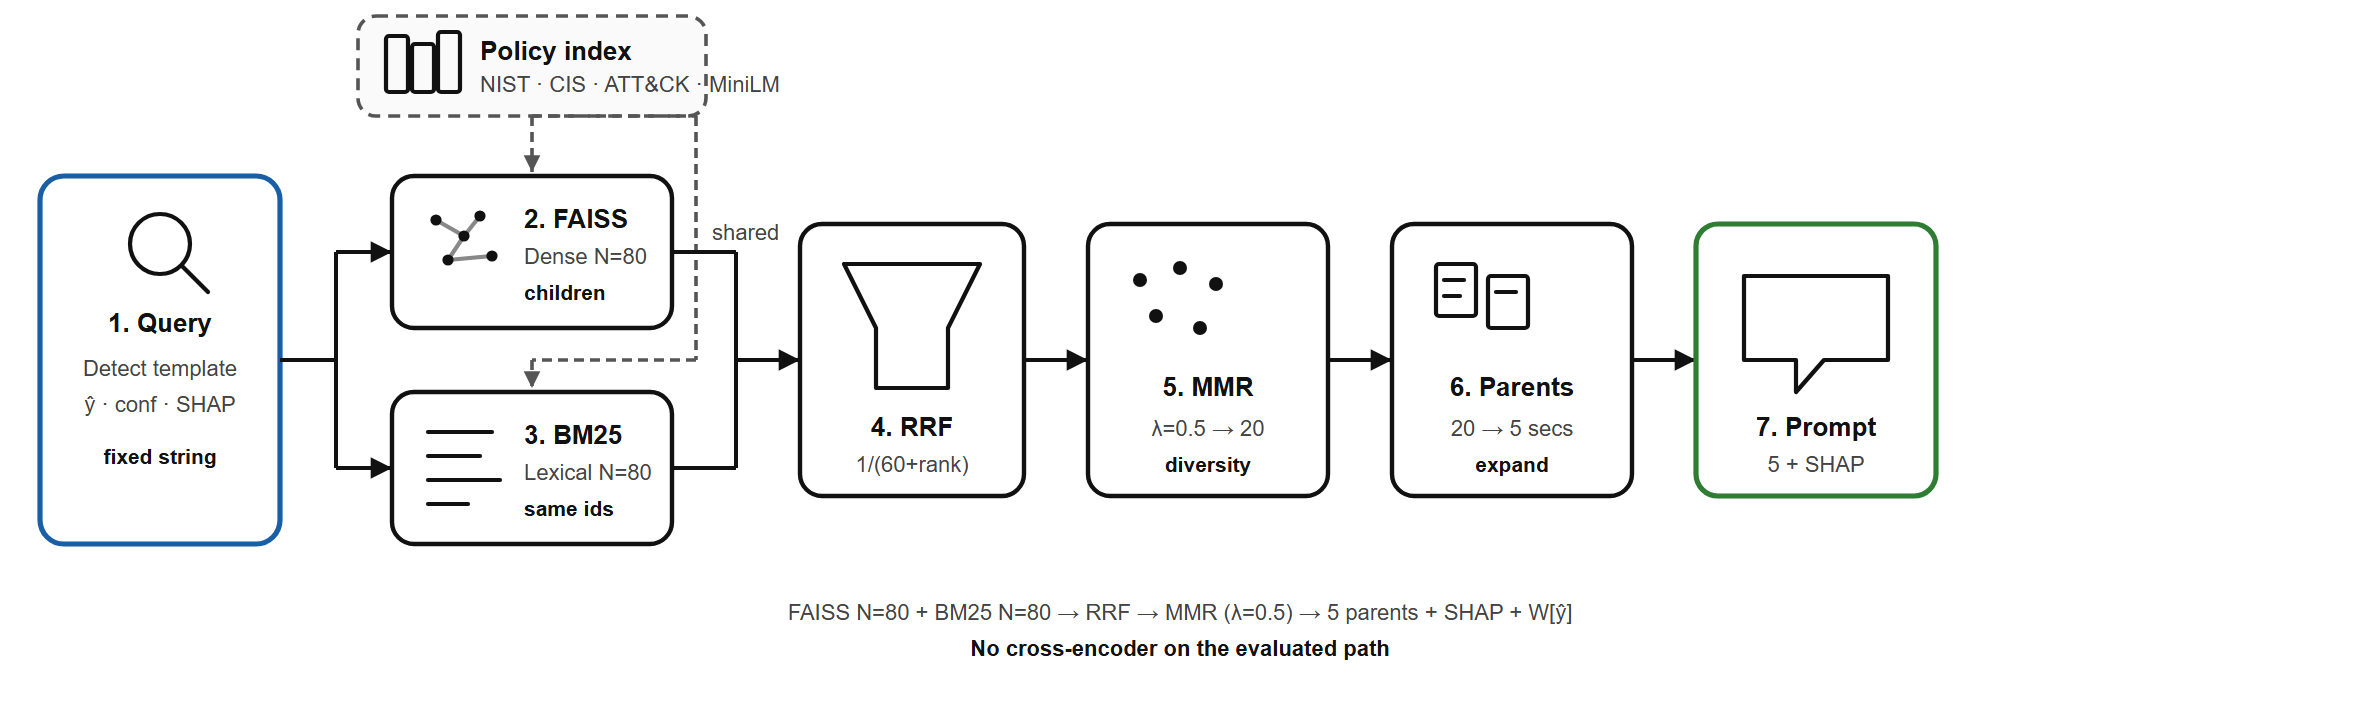
\includegraphics[width=\columnwidth]{retrieval_pipeline_v5.png}
    \caption{RAG retrieval and context construction pipeline.}
    \label{fig:rag-retrieval}
\end{figure}

\begin{enumerate}
\item \emph{Dense retrieve (recall).} FAISS returns an oversampled neighbor list ($\min(300,\,20\times 6)$), keeps $20$ children, converts distance $d$ to similarity $1/(1+d)$, and balances hits across source files so one document cannot occupy the entire top-$20$. The bi-encoder is cheap and high-recall; it is not a relevance judge.
\item \emph{Merge and dedupe.} Multi-query children are unioned by $(\mathrm{parent\_id},\,\mathrm{child\_index})$ (else source, title, and a short prefix). The higher similarity wins. Without this step, overlap would inject the same passage twice and starve the later budget.
\item \emph{MMR (diversity).} Maximum Marginal Relevance with $\lambda=0.5$ keeps up to $60$ children,
\begin{equation}
\mathrm{MMR}(c)=\lambda\cdot\mathrm{sim}(q,c)-(1-\lambda)\cdot\max_{c'\in S}\mathrm{sim}(c,c').
\label{eq:mmr}
\end{equation}
After merge the pool is still redundant; without MMR the cross-encoder would re-score the same control and NIST, CIS, and ATT\&CK would not coexist in the prompt.
\item \emph{Cross-encoder (precision).} Each surviving $(q,\mathrm{passage})$ pair is scored jointly by \texttt{cross-encoder/ms-marco-MiniLM-L-6-v2} (passage truncated at $4000$ characters) and sorted. Vector similarity is a topical neighborhood, not ``this passage is a mitigation for \emph{this} PortScan at the perimeter.'' The cross-encoder is the relevance model; it is too expensive to run on the whole index, which is why steps 1--3 exist.
\item \emph{Rerank cut.} The top $20$ children by cross-encoder score are kept.
\item \emph{Parent expansion.} Each kept child is replaced by its parent section (capped at $12\,000$ characters); duplicate parents collapse to the higher child score. The planner must quote a control, not a $384$-character shard.
\item \emph{Prompt budget.} The top five sections (up to ten) are emitted as numbered $[k]$ title + body + source. If the list is empty, the slot is the explicit sentence that no relevant documents were found, and the model is forbidden to invent policy.
\end{enumerate}
Retrieval returns guidance and allowable primitives. It does not invent action names. The closed list $W[\hat{y}_i]$ is supplied in a different prompt slot and is the only legal vocabulary for \texttt{action}---the same catalog the Blockchain Governance Layer will store as an unpromptable whitelist~\cite{jan2025,karim2025}.

As shown in Fig.~\ref{fig:rag-retrieval}, dense retrieval over the FAISS index is followed by MMR diversification and cross-encoder re-ranking to construct the final context.

\paragraph{Prompt Construction.}
The prompt construction process is illustrated in Fig.~\ref{fig:prompt-construct}.
The user message is one template whose slots are filled in software before any decode~\cite{xi2023,li2025}. The model never sees raw telemetry, never sees the $192$-dimensional fusion vector, and never sees action names outside $W[\hat{y}_i]$. The slots are: (i)~role and the three exact domain strings; (ii)~prediction summary ($\hat{y}_i$, $\mathrm{conf}_i$); (iii)~the dominance sentence produced from $p_i^{\star}$; (iv)~the Detection evidence JSON, top-$5$ features only; (v)~$W[\hat{y}_i]$ plus preferred domains and typical evidence cues for that class; (vi)~a per-domain card (role, top-$3$ features, actions that domain is allowed to execute---the intersection of class whitelist and domain capability); (vii)~the numbered RAG sections, or the empty-KB sentence. The task block, also template text, requires the model to interpret $\hat{y}_i$ on all three domains, name which domain must act first, select actions only from the list, assign each a network tier, cite evidence in per-action reasoning, scale execution priority with $\mathrm{conf}_i$, and return empty lists rather than a made-up control if nothing fits. Decoding uses GPT-4o-mini at temperature $T=0.3$ with the instruction to return only valid JSON; the first ``\{'' through the last ``\}'' is parsed and surrounding prose is discarded.



\begin{figure*}[!t]
\centering
\includegraphics[width=\textwidth]{llm_prompt_template.png}
\caption{Prompt construction format. The user message is Role (fixed) plus eight runtime slots filled in software before decode, plus a required JSON response schema. GPT-4o-mini at $T=0.3$; action names must occur in $W[\hat{y}_i]$; $\mathtt{network\_tier}$ is exactly Access~/~ISP, Perimeter~/~IDS, or Endpoint~/~EDR.}
\label{fig:prompt-construct}
\end{figure*}

\paragraph{Response Schema.}
The only accepted output is one object $\mathrm{plan}_i$ (Table~\ref{tab:plan-schema}). The field \texttt{action} is copied from $W[\hat{y}_i]$, not paraphrased (\texttt{limit rate} remains \texttt{limit rate}). \texttt{network\_tier} is exactly one of the three domain strings. Primary actions prefer $p_i^{\star}$ unless the evidence contradicts it. Empty RAG forbids invented policy citations. A PortScan whose Perimeter share dominates is therefore planned as, for example, \texttt{tarpit scan} and \texttt{harden ports} at Perimeter~/~IDS with a supporting \texttt{update ACL} at Access~/~ISP---names that are legal for PORTSCAN and illegal for BENIGN~\cite{sharafaldin2018}. That legality is not left to the model: Apply will reject any name that is absent from $W[\hat{y}_i]$ or absent from this object.

% preamble: \usepackage{booktabs,tabularx,ragged2e}

\begin{table}[t]
\caption{Mitigation Plans object $\mathrm{plan}_i$. Action names must occur in $W[\hat{y}_i]$; \texttt{network\_tier} must be one of the three enterprise domains.}
\label{tab:plan-schema}
\centering
\small
\setlength{\tabcolsep}{4pt}
\renewcommand{\arraystretch}{1.1}
\begin{tabularx}{\columnwidth}{@{}>{\RaggedRight\arraybackslash}p{0.34\columnwidth}>{\RaggedRight\arraybackslash}X@{}}
\toprule
\textbf{Field} & \textbf{Constraint} \\
\midrule
\texttt{threat\_\allowbreak level} & Critical, High, Medium, or Low \\
\texttt{all\_\allowbreak actions} & Union of primary and supporting action names \\
\texttt{primary\_\allowbreak actions}[] & Action units with \texttt{action}, \texttt{network\_\allowbreak tier}, \texttt{party\_\allowbreak evidence\_\allowbreak type}, and \texttt{reasoning} \\
\texttt{supporting\_\allowbreak actions}[] & Same shape as primary units \\
\texttt{overall\_\allowbreak reasoning} & Why this Access~/~Perimeter~/~Endpoint order \\
\texttt{execution\_\allowbreak priority} & Immediate, High, Standard, or Low \\
\texttt{knowledge\_\allowbreak sources\_\allowbreak used} & Catalog and/or retrieved-section tags \\
\bottomrule
\end{tabularx}
\end{table}



\paragraph{Handoff to Blockchain Governance.}
$\mathrm{plan}_i$ is this layer's only output. Reason never calls the contract and never opens a device API. This closes the evidence-to-plan failure that Section~\ref{sec:detect} left open: the planner cannot speak an action that is not in the catalog, cannot omit a domain assignment, and cannot hide the Detection fields it used. It does not close the trust failure that follows generation~\cite{chhabra2026,pendli2025}. A fluent, catalog-legal action copied from another cycle, or a unit whose network tier is rewritten after decode, will still look like a valid plan if the next layer only stores private text. Binding $W[\hat{y}_i]$ on-chain, writing each $\{u,\tau\}$ once, and refusing any apply that is not an exact unit in that record is the failure the Blockchain Governance Layer exists to close~\cite{zhang2024exploit,jan2025}.

\subsubsection{Blockchain Governance Layer (Commit)}
\label{sec:commit}

What fails without this layer: Reasoning is probabilistic. A language model can emit a fluent action that is still harmful on a live path, and a substituted plan can change between generation and dispatch. A policy paragraph in a prompt is not a control: it can be ignored, reworded, or overwritten. Autonomous defense therefore needs a pre-execution governance layer that cannot hallucinate mitigations and cannot be talked into accepting them~\cite{karim2025,pendli2025,lazer2026,chhabra2026}.

The registry \texttt{AgenticTrustRegistry} uses the ledger for two jobs: an unpromptable per-attack whitelist $W$, and a write-once, readable record of the plan produced for this detection cycle~\cite{jan2025,zhang2024exploit}. It does not classify traffic, does not retrieve policy, does not re-detect the flow, and does not dispatch. Those remain Detect, Reason, and Apply.

\paragraph{Off-Chain Artifact versus On-Chain Record.}
After Reason returns, the full Mitigation Plans object---prompt, RAG passages, and free-form reasoning---stays off-chain in MySQL and JSON. Commit writes only the fields an execution gate must check without reconstructing the prompt: identities ($\mathit{jobId}$, $\mathit{predictionId}$, $\mathit{rowIndex}$); $\mathit{attackType}$ and $\mathit{threatLevel}$; primary and supporting units, each $\{u,\tau\}$ with $\tau\in\{\text{Access~/~ISP},\ \text{Perimeter~/~IDS},\ \text{Endpoint~/~EDR}\}$; and
\begin{equation}
h=\mathrm{SHA256}(\texttt{overall\_reasoning}),
\label{eq:reasoning-hash}
\end{equation}
the only digest on the ledger. Telemetry, the $192$-d fusion vector, SHAP tables, and LLM prose never enter the contract. Attack type, threat, and action units are stored as plain text, so Apply reads them with \texttt{getPlan} and \texttt{isInPlan}$(\mathit{planId},u,\tau)$ rather than re-hashing a private JSON blob. $\mathit{planId}$ is the agentic report identity, not the job identity: one agentic job can produce several plans.

\begin{table}[t]
\caption{On-chain fields after \texttt{storePlan}. Catalog fields are plaintext; only reasoning is hashed.}
\label{tab:onchain-plan}
\centering
\begin{tabular}{p{0.28\columnwidth}p{0.64\columnwidth}}
\hline
Field & Example (PortScan) \\
\hline
\texttt{planId} & agentic report identity \\
Detect link & \texttt{jobId}, \texttt{predictionId}, \texttt{rowIndex} \\
\texttt{attackType} / \texttt{threatLevel} & PORTSCAN / High \\
primary units & $\{\texttt{tarpit scan},\ \text{Perimeter~/~IDS}\}$, $\{\texttt{harden ports},\ \text{Perimeter~/~IDS}\}$ \\
supporting units & $\{\texttt{update ACL},\ \text{Access~/~ISP}\}$ \\
\texttt{reasoningHash} & SHA-256 of \texttt{overall\_reasoning} \\
\texttt{origin} / parent & \texttt{agent} / empty \\
\texttt{superseded} & false \\
\hline
\end{tabular}
\end{table}

\paragraph{Policy Whitelist.}
At deploy, the owner seeds $W[a,u]$ from the same constrained catalog Reason was allowed to name (Table~\ref{tab:whitelist}). After seed, ordinary callers cannot add a name. $W$ does not depend on the prompt. An action that is legal for DDoS and illegal for the predicted PortScan fails even if the sentence is fluent: the model cannot talk a new token onto $W$. Tiers and threat levels are closed sets; each action list is capped at ten units; a duplicate $\{u,\tau\}$ is rejected.

\paragraph{Write-Once Plan Record.}
\texttt{storePlan}$(\mathit{planId},\mathrm{Plan})$ may be called only by an authorized planner. It requires a known attack type, a valid threat level, a nonempty $h$, and that every unit already sits on $W$. A second write to the same $\mathit{planId}$ is rejected. The transaction emits \texttt{PlanStored}. Later readers call \texttt{getPlan} and \texttt{isInPlan}. Three outcomes are distinguishable: (i)~the on-chain action list matches the off-chain file---this is the committed plan; (ii)~the file names a different action or tier---substitution, so Apply must not proceed; (iii)~the plan is missing or \texttt{superseded}---the cycle is not live.

\paragraph{Authorized Callers.}
The owner authorizes planner keys, reviewer keys, and one executor key per network tier. Planners store an original plan (\texttt{origin}=\texttt{agent}). They do not mark actions applied. D1 (Access~/~ISP), D2 (Perimeter~/~IDS), and D3 (Endpoint~/~EDR) each have a distinct executor: only that key may later receipt a unit on its tier. An Access action cannot be marked applied by the Endpoint executor.

\paragraph{Human Correction, Not Re-Detection.}
If Apply later finds a mismatch (\texttt{action\_not\_whitelisted} or \texttt{action\_plan\_mismatch}), Detect is not run again. A reviewer calls \texttt{revisePlan}$(\mathit{newId},\mathit{parentId},\mathrm{Plan})$ with a corrected $\{u,\tau\}$ list that keeps the parent's $\mathit{predictionId}$, $\mathit{rowIndex}$, and $\mathit{attackType}$. The parent is marked \texttt{superseded} and can no longer be applied. Origin is \texttt{human}. An authorized agent may revise an original \texttt{agent} plan once (\texttt{origin}=\texttt{replan}); any further correction must come from a reviewer. The new $\mathit{planId}$ is the only live record Apply will accept.

\paragraph{Governance as a Signal, Not an Actuator.}
\texttt{PlanStored} and \texttt{PlanRevised} are tamper-evident events that a validated, or human-corrected, proposal exists. A SOC, SIEM, or ticket queue may subscribe. The architecture does not require a vendor-specific SOC. The contract freezes what may be done; it does not open API, gRPC, or MCP~\cite{chen2024,jin2024}.

This closes the ungoverned-proposal problem, but a frozen plan is still not an actuation. A still-whitelisted action copied from another cycle, a unit whose domain no longer matches the plan, or a superseded parent must be refused at the point of execution. Checking $W$, \texttt{isInPlan}, the live $\mathit{planId}$, and the tier executor key, then posting that unit to D1, D2, or D3, is the failure the next layer exists to close.

\subsubsection{Execution and Monitoring Layer (Apply)}
\label{sec:apply}

Once Commit has written a live $\mathit{planId}$, the pipeline does not wait for a separate orchestrator. The Blockchain Governance layer hands that record directly to the execution-monitoring agent, which is the only process allowed to open a device interface. The agent's job is narrow: confirm that $\{u,\tau\}$ is still authorized, try to run it, and then either close the loop with an operator or write the outcome into the operational store (Fig.~\ref{fig:system_diagram}).

\begin{figure}[H]
    \centering
    \includegraphics[width=\columnwidth]{blockchain_flow.png}
    \caption{Human-in-the-loop Apply. A gate or device miss is logged and the
    operator revises the plan; a successful call is receipted on-chain and in
    the database / SOC / log. Detect is not rerun.}
    \label{fig:blockchain_flow}
\end{figure}

\paragraph{Execution Gate.}
No API, gRPC, or MCP call is issued until three on-chain tests succeed, in this order. First, $u$ must sit on the per-attack whitelist $W[a]$; a fluent name that Reason never had permission to emit dies here, as does a DDoS primitive offered against a PortScan. Second, the pair $\{u,\tau\}$ must be in the live plan (\texttt{isInPlan}): a still-legal action copied from another cycle, or the same action aimed at a different domain, is a mismatch. Third, the plan must not be \texttt{superseded}; after a human revision the parent can no longer be applied. Compactly,
\begin{equation}
W[a,u]=1 \;\wedge\; \{u,\tau\}\in\mathrm{plan}(\mathit{planId}) \;\wedge\; \neg\mathrm{superseded}(\mathit{planId}).
\label{eq:apply-gate}
\end{equation}
\texttt{markApplied} repeats the same checks and additionally requires that the caller is the executor key for $\tau$. Software can fail closed before the transaction; the contract is the second lock.

\paragraph{Per-Attack Whitelist.}
Table~\ref{tab:whitelist} is the catalog $W$ already seeded at Commit. Apply does not enlarge it.

\begin{table}[t]
\caption{Per-attack action whitelist $W$ at Apply time. Labels follow CICIDS-2017~\cite{sharafaldin2018}; actions are a constrained catalog, not free-form LLM text.}
\label{tab:whitelist}
\centering
\begin{tabular}{p{0.28\columnwidth}p{0.64\columnwidth}}
\hline
Attack $a$ & Allowed actions (excerpt) \\
\hline
BENIGN & log incident, monitor traffic \\
DDOS~/~DOS & limit rate, enable scrubbing, block IP, enable syncookies, update ACL \\
SSHPATATOR~/~FTPPATATOR & fail2ban block, lock account, enforce MFA \\
PORTSCAN & tarpit scan, harden ports, update ACL \\
WEBATTACK & apply WAF, virtual patch, isolate service \\
BOT & captcha challenge, reputation filter \\
OTHERS & log incident, isolate service, update ACL \\
\hline
\end{tabular}
\end{table}

\paragraph{Dispatch to the Domain Agent.}
A unit that passes the gate is sent to the executor of its tier: D1 (Access~/~ISP) at the ISP-edge / ACL controller, D2 (Perimeter~/~IDS) at the firewall / IDS / WAF, or D3 (Endpoint~/~EDR) at host isolation. The call is API, gRPC, or MCP, with payload $\{u,\tau,\hat{y}_i,\mathit{planId}\}$. D2 never receives an Endpoint unit~\cite{chen2024,jin2024}. The evaluated build records that attempt; production replaces the stub URL with the live control plane.

\paragraph{Human in the Loop.}
A miss---whitelist, plan-binding, superseded parent, device timeout, or a rejected control---does not re-enter Detect and does not mark the unit applied. The execution-monitoring agent writes a structured failure record ($\mathit{planId}$, $\{u,\tau\}$, reason, timestamp) to the log and notifies the operator that the plan needs an update. That is the human-in-the-loop: the operator edits only the action list and domains, keeping the same $\mathit{predictionId}$, $\mathit{rowIndex}$, and $\hat{y}_i$, then calls \texttt{revisePlan} (Section~\ref{sec:commit}). The parent is superseded; origin is \texttt{human}; Apply retries on the new $\mathit{planId}$. The operator cannot skip Eq.~(\ref{eq:apply-gate}), cannot add a name that is not on $W$, and cannot point a Perimeter action at D3. A single agent replan is allowed on an original \texttt{agent} plan; any further correction is reviewer-only (Fig.~\ref{fig:blockchain_flow}).

\paragraph{Success Path.}
When the device call returns success, the executor of $\tau$ issues \texttt{markApplied} and emits \texttt{ActionApplied}. The same receipt is written to the database execution report, the SOC / SIEM bus, and the monitoring log. A second apply of that $\{u,\tau\}$ on this $\mathit{planId}$ is refused.

\begin{algorithm}[t]
\caption{Commit and Apply}
\label{alg:commit-apply}
\begin{algorithmic}[1]
\PROCEDURE{Commit}{$\mathit{planId}$, $\mathrm{Plan}$}
    \STATE \textbf{require} $\mathit{planId}$ not already stored
    \STATE \textbf{require} attack $a$ known, threat valid, $h\neq 0$
    \FOR{each unit $\{u,\tau\}$ in $\mathrm{Plan}$}
        \STATE \textbf{require} $W[a,u]=1$ \COMMENT{policy ground}
        \STATE \textbf{require} $\tau\in\{\text{Access},\text{Perimeter},\text{Endpoint}\}$
    \ENDFOR
    \STATE store plaintext $\mathrm{Plan}$; emit \texttt{PlanStored}
\ENDPROCEDURE
\PROCEDURE{Revise}{$\mathit{newId}$, $\mathit{parentId}$, $\mathrm{Plan}$}
    \STATE \textbf{require} parent exists and is not superseded
    \STATE \textbf{require} same $\mathit{predictionId}$, $\mathit{rowIndex}$, and $a$ as parent
    \STATE call \textsc{Commit}($\mathit{newId}$, $\mathrm{Plan}$) \COMMENT{human-in-the-loop}
    \STATE mark parent superseded; emit \texttt{PlanRevised}
\ENDPROCEDURE
\PROCEDURE{Apply}{$\mathit{planId}$, $u$, $\tau$}
    \STATE \textbf{require} plan exists and is not superseded
    \STATE \textbf{require} $W[a,u]=1$ \COMMENT{policy ground}
    \STATE \textbf{require} $\{u,\tau\}\in\mathrm{plan}(\mathit{planId})$ \COMMENT{plan binding}
    \STATE \textbf{require} caller is the executor of $\tau$
    \STATE try API / gRPC / MCP to D1, D2, or D3 according to $\tau$
    \IF{dispatch fails}
        \STATE log the failure; notify operator to update the plan
        \STATE \textbf{return} \COMMENT{no \texttt{markApplied}; Detect is not rerun}
    \ENDIF
    \STATE mark applied; emit \texttt{ActionApplied}
    \STATE write success to database, SOC, and log
\ENDPROCEDURE
\end{algorithmic}
\end{algorithm}

Apply therefore sits between a frozen ledger and a live network. The agent tries the gated call; if the network or the gate says no, a person revises the plan and the same checks run again; if the call succeeds, the database, the SOC, and the chain all see the same receipt. The language model is not asked to recover, and Detect is not asked to look at the flow a second time.



%===========================

\section{Experimental Setup and Implementation}
\label{sec:setup}

We evaluate our system on CICIDS-2017~\cite{sharafaldin2018} using the complete Detect--Reason--Commit--Apply pipeline described in Section~\ref{sec:system}. The evaluation covers three aspects: (i) intrusion-detection performance of the three-party VFL model, (ii) apply-time enforcement against modified mitigation actions, and (iii) blockchain processing overhead. The implementation integrates PyTorch-based VFL and SHAP, a RAG-grounded LLM planner, MySQL/JSON persistence, and the \texttt{AgenticTrustRegistry} smart contract into a single executable stack.

\begin{table*}[t]
\centering
\small
\renewcommand{\arraystretch}{1.4}
\setlength{\tabcolsep}{6pt}
\caption{Pipeline stages and configuration.}
\begin{tabularx}{\textwidth}{|p{2.4cm}|p{3.4cm}|X|}
\hline
\rowcolor
\hcell{Stage} & \hcell{Component} & \hcell{Configuration} \\
\hline

\textbf{1 DETECT} &
Local Encoder &
$d_p \rightarrow 128 \rightarrow 64$, dropout 0.2 / 0.1 ($\times$ 3 parties) \\
\hline

&
Fusion + Classifier &
concat $h \in \mathbb{R}^{192} \rightarrow 192 \rightarrow 128 \rightarrow K$,
dropout 0.2 \\
\hline

&
Attribution &
KernelSHAP on distilled surrogate, $T{=}3.0$, 100 background / 200 perturbations \\
\hline

&
Training &
Adam (lr $10^{-3}$, wd $10^{-4}$), class-weighted CE (clamp $20\times$),
early stopping (patience 20), 100 epochs \\
\hline

\textbf{2 REASON} &
Query + Retrieval &
FAISS, chunk 512 / overlap 64, all-MiniLM-L6-v2, cross-encoder reranking \\
\hline

&
LLM Agent &
GPT-4o-mini, $T=0.3$, deterministic JSON schema \\
\hline

&
Constraint &
Every action $\in$ whitelist $W[\hat{y}]$;
network\_tier $\in \{\mathrm{Access},\mathrm{Perimeter},\mathrm{Endpoint}\}$ \\
\hline

\textbf{3 COMMIT} &
Canonicalization &
$P$ = identity + retrieval context + plan + assigned tiers \\
\hline

&
Smart Contract &
AgenticTrustRegistry.sol, Solidity 0.8.20, write-once \texttt{anchor()} \\
\hline

&
Whitelist &
$W[a,u]$, seeded per attack class from policy \\
\hline

\textbf{4 APPLY} &
Execution Gate &
$W[\hat{y},u]{=}1 \;\wedge\; u \in \mathrm{plan}(P)
\;\wedge\;$ on-chain digest $= \mathrm{rehash}(P)$ \\
\hline

&
Dispatch &
API / gRPC / MCP, signed gated call \\
\hline

&
Audit + Reject &
Every hop logged; rejected $\rightarrow$ operator review;
approval re-anchors \\
\hline

\textbf{SETUP} &
Feature Partition &
D1 Access/ISP: 23 cols $\cdot$
D2 Perimeter/IDS: 32 cols $\cdot$
D3 Endpoint/EDR: 42 cols \\
\hline

&
Dataset &
CICIDS-2017, 390,398 flows, stratified 64/16/20 split, seed 42 \\
\hline

&
Blockchain Environment &
Hardhat 2.22 (chain ID 31337), solc 0.8.24, 200 optimizer runs \\
\hline

\end{tabularx}

\label{tab:pipeline}
\end{table*}



\subsection{Dataset and Preprocessing}

The experiments use a prepared CICIDS-2017 dataset containing $390{,}398$ labeled network-flow records. After preprocessing, $88$ numeric traffic features are retained for model development. Non-predictive identifiers such as flow identifiers, source/destination addresses, and timestamps are excluded when present, and only numeric flow attributes are supplied to the learning pipeline.

The original CICIDS attack labels are consolidated into nine classes:
\texttt{BENIGN}, \texttt{BOT}, \texttt{DDOS}, \texttt{DOS},
\texttt{FTPPATATOR}, \texttt{OTHERS}, \texttt{PORTSCAN},
\texttt{SSHPATATOR}, and \texttt{WEBATTACK}. Related attack variants are merged into their common parent classes; for example, the DoS variants are grouped as \texttt{DOS}, while Web Attack variants are represented as \texttt{WEBATTACK}. Classes containing fewer than $200$ observations are grouped into \texttt{OTHERS}; in the prepared dataset, \texttt{INFILTRATION} ($122$ flows) and \texttt{HEARTBLEED} ($70$ flows) form this category.

The resulting data are divided using stratified sampling with random seed $42$. We use $64\%$ for training ($249{,}854$ flows), $16\%$ for validation ($62{,}464$ flows), and $20\%$ for testing ($78{,}080$ flows). Stratification preserves the class distribution across all three splits. Features assigned to each VFL participant are standardized using \texttt{StandardScaler} and converted to 32-bit floating-point tensors before training.


\subsection{VFL Model and Training Configuration}
VFL and the centralized baseline use identical optimization so that differences reflect the architecture, not the training setup. We use class-weighted cross-entropy, with inverse-frequency weights clamped at $20\times$ to prevent rare classes from dominating the gradient. Optimization uses Adam ($\mathrm{lr}=10^{-3}$, weight decay $10^{-4}$) with gradient clipping at $\ell_2=1$, and a plateau scheduler that halves the learning rate on validation stall (factor $0.5$, patience $15$, floor $10^{-6}$). Training runs up to $100$ epochs, validates every $5$ epochs, and early-stops on macro-$F_1$ (patience $20$, $\Delta_{\min}=0.001$), restoring the best checkpoint. We report accuracy, macro-recall, macro-$F_1$, and a per-class comparison against the centralized model.

\subsection{Centralized All-Feature Baseline.}
A privacy-preserving claim is meaningful only if VFL is compared against a model with full feature access~\cite{ye2024vfl,yu2024vflprivacy}. We therefore concatenate the three scaled feature slices into $\tilde{x}_i = [x_i^1 \| x_i^2 \| x_i^3] \in \mathbb{R}^{d}$ and train a non-federated MLP of comparable depth ($d \to 256 \to 128 \to 64 \to K$, ReLU and dropout $0.2$ at each hidden layer), using the same split, class weights, optimizer, scheduler, and early-stopping rule. The depth is deliberate: a weaker baseline would make VFL look favorable for the wrong reason. This centralized model is an evaluation instrument only---it is not deployed, does not produce SHAP explanations, and does not feed Reason. The live pipeline uses VFL embeddings exclusively.

\subsection{Explainability and RAG Configuration}

After detection, KernelSHAP is applied to the fused $192$-dimensional representation to obtain domain- and feature-level contributions. The predicted class, confidence, and SHAP evidence are then passed to the RAG pipeline. Security documents are split into chunks of $512$ with an overlap of $64$, embedded using \texttt{all-MiniLM-L6-v2}, and indexed in FAISS. The top-$5$ retrieved passages are reranked using a cross-encoder and provided with the SHAP context to GPT-4o-mini, which generates a structured mitigation plan constrained by the predefined action catalog.

\subsection{Blockchain and Implementation Stack}

The governance component is implemented through
\texttt{AgenticTrustRegistry.sol} using Solidity~0.8.20. Experiments use a local Hardhat~2.22 Ethereum-compatible network with chain ID~$31337$. The contract is compiled using \texttt{solc}~0.8.24 with optimization enabled for $200$ runs, and the backend interacts with the ledger through Web3.py and JSON-RPC.

After Reason produces a mitigation plan, the complete artifact remains off-chain in MySQL and JSON storage. The backend canonicalizes the corresponding payload $P$ and computes
\[
c=\mathrm{SHA256}(P).
\]
Only the resulting \texttt{bytes32} commitment is stored on-chain through \texttt{anchor}. Raw network features, SHAP evidence, retrieved policy passages, and human-readable LLM output are therefore not stored on the blockchain. The contract additionally maintains the per-attack action whitelist and the state of successfully applied actions.

At Apply, \texttt{getCommitment} retrieves the stored commitment and the persisted payload is re-hashed before an action is admitted. The execution path then applies the two checks : the action must be permitted by the whitelist for the detected attack class and must belong to the plan committed for the current detection cycle. A successful unit is recorded through \texttt{applyAction}.

\begin{table}[t]
\centering
\caption{ Host and Implementation stack.}
\label{tab:stack}
\setlength{\tabcolsep}{4pt}
{\footnotesize
\begin{tabular}{@{}lp{5.0cm}@{}}
\hline
\textbf{Component} & \textbf{Configuration} \\
\hline
OS / CPU & Windows 10 Pro 64-bit; Intel i5-8365U, 4C/8T, 1.60\,GHz \\
RAM / GPU & 16\,GB; Intel UHD 620; no CUDA \\
Runtime & Python 3.11+; Node.js 22 \\
Detection & PyTorch; VFL; KernelSHAP \\
Database & MySQL 8; JSON artifact storage \\
RAG & LangChain; FAISS; MiniLM; cross-encoder \\
LLM & GPT-4o-mini ($T\approx0.3$) \\
Backend / UI & FastAPI / React \\
Contract & \texttt{AgenticTrustRegistry}, Solidity 0.8.20 \\
Compiler & \texttt{solc} 0.8.24; optimizer, 200 runs \\
Blockchain & Hardhat 2.22; chain ID $31337$ \\
Client & Web3.py; JSON-RPC \\
Commitment & SHA-256 of canonical JSON; \texttt{bytes32} on-chain \\
\hline
\end{tabular}}
\end{table}

\subsection{System Evaluation}

The system is evaluated end-to-end using $500$ CICIDS-style network flows submitted sequentially through the live backend API. Each flow passes through the Detect--Reason--Commit--Apply pipeline while the trained VFL model, FAISS index, MySQL database, and Hardhat blockchain remain active throughout the run.

To test enforcement integrity, selected actions are modified after Commit but before Apply. The modifications include either actions that are invalid for the detected class or whitelist-valid actions that were not part of the committed plan. Apply then evaluates the whitelist and plan-binding gates to determine whether the modified actions are rejected.

The current executor records execution receipts rather than invoking a live network device. A production deployment can replace this stub with an API, MCP interface, SOAR playbook, or SDN controller without changing the validation gates. The implementation is available at
\url{https://github.com/sharif2008/pragma}.




%=================================================================
\section{Experimental Results and Analysis} \label{sec:results}
We evaluated the proposed system in three settings: detection quality; enforcement performance, including execution behavior and blockchain latency; and a stage-wise ablation of end-to-end Detect--Reason--Commit--Apply latency. Detection quality was measured on the held-out CICIDS-2017 test set ($N{=}78{,}080$ flows across nine classes). As shown in Table~\ref{tab:vfl}, the three-party Vertical Federated Learning (VFL) model achieves an accuracy of $0.9628$, macro-recall of $0.9861$, and macro-F1 of $0.8633$, compared with $0.9614$, $0.9829$, and $0.8617$, respectively, for the centralized MLP trained on all $88$ features. The macro-F1 difference is only $0.0016$, indicating that feature locality is achieved without materially degrading detection performance. The objective of vertical partitioning is therefore privacy-preserving feature locality rather than an accuracy gain over centralized learning.

\begin{table}[t]
\centering
\caption{Detection Performance on CICIDS-2017 (78{,}080 Samples, 9 Classes)}
\label{tab:vfl}
\renewcommand{\arraystretch}{1.2}
\begin{tabular}{@{}lccc@{}}
\toprule
\textbf{Model} & \textbf{Acc.} & \textbf{Mac.\ Rec.} & \textbf{Mac.\ F1}\\
\midrule
VFL (3 parties, strict locality)    & 0.9628 & 0.9861 & 0.8633\\
Standard NN (centralized, 88 feat.) & 0.9614 & 0.9829 & 0.8617\\
\midrule
Difference (VFL $-$ NN)             & +0.0014 & +0.0032 & +0.0016\\
\bottomrule
\end{tabular}
\end{table}


We ingested 500 network flows through the live API, drawn as a 5\% stratified sample per class from a pool of 1{,}000 records, ensuring proportional representation across all nine attack labels listed in Table~\ref{tab:enforce}. Before the first flow was processed, the API was initialized with the trained three-party VFL model, MySQL, FAISS, and a local Hardhat node (chain ID $31337$) with a seeded \texttt{AgenticTrustRegistry}. Each CICIDS-style feature vector was submitted over HTTP, one flow at a time, emulating how a monitoring component would ingest individual sensor events through \texttt{attack\_monitor.py}. The experiment therefore evaluates online, row-by-row processing of the deployed stack rather than packet capture from a live network interface.

For each flow, Detect scores the input using the VFL model, applies KernelSHAP, and maps the predicted label to its corresponding policy in Table~\ref{tab:whitelist}. Reason retrieves the relevant RAG context, after which GPT-4o-mini generates a structured mitigation plan containing an average of $3.08$ action units per flow. Commit canonicalizes the resulting plan and stores its SHA-256 digest on-chain through \texttt{anchor}, creating a tamper-evident commitment to the proposed actions.

For the enforcement experiment, the $500$-flow run was executed with \texttt{--tamper} enabled. Before Apply, the client modifies either one or two action units per flow, alternating according to row index while leaving the remaining actions unchanged. Each modification represents one of two threat cases derived from Table~\ref{tab:whitelist}: either an action permitted for another attack class but not for the current class, or an action that remains valid under the current class whitelist but was not part of the committed plan. Apply submits the resulting mixed action list, after which the two gates in Eq.~(\ref{eq:apply}) are evaluated sequentially: first the class-specific whitelist check and then the plan-binding check. An action unit that passes both gates is recorded through \texttt{applyAction}.

Table~\ref{tab:enforce} reports the execution outcome for each attack class. Across the $500$ flows, the Reason stage generated $1538$ action units, of which $750$ were deliberately modified. Gate~1 rejected $352$ off-whitelist substitutions with \texttt{action\_not\_whitelisted}, while Gate~2 rejected the remaining $398$ substitutions with \texttt{action\_plan\_mismatch}. Thus, all $750$ modified units were rejected, while the $788$ unchanged units successfully received execution receipts. The results demonstrate the complementary roles of the two enforcement gates: Gate~1 prevents actions that violate class-specific policy, whereas Gate~2 detects substitutions that remain policy-valid but differ from the committed mitigation plan.

\begin{table}[t]
\centering
\caption{Per-class execution outcome on $500$ online flows with \texttt{--tamper}.
Every changed unit is refused (Block.\% ${=}100$).
WL $=$ whitelist reject; Plan $=$ plan-list reject; Applied $=$ unmodified receipts.}
\label{tab:enforce}
\setlength{\tabcolsep}{3.5pt}
{\footnotesize
\begin{tabular}{@{}lrrrrrrr@{}}
\hline
Attack & $n$ & Proposed & Changed & WL & Plan & Applied & Block.\% \\
\hline
BENIGN & 41 & 82 & 60 & 29 & 31 & 22 & 100 \\
BOT & 37 & 87 & 59 & 27 & 32 & 28 & 100 \\
DDOS & 35 & 107 & 55 & 26 & 29 & 52 & 100 \\
DOS & 126 & 357 & 185 & 80 & 105 & 172 & 100 \\
FTPPATATOR & 37 & 188 & 56 & 27 & 29 & 132 & 100 \\
OTHERS & 60 & 183 & 91 & 47 & 44 & 92 & 100 \\
PORTSCAN & 31 & 90 & 49 & 23 & 26 & 41 & 100 \\
SSHPATATOR & 30 & 148 & 46 & 20 & 26 & 102 & 100 \\
WEBATTACK & 103 & 296 & 149 & 73 & 76 & 147 & 100 \\
\hline
Total & 500 & 1538 & 750 & 352 & 398 & 788 & 100 \\
\hline
\end{tabular}}
\end{table}

In the testbed, the final executor is implemented as a stub that records only the execution receipt. In a production SOC environment, this component can be replaced by an operational interface such as an API call, MCP tool, SOAR playbook, or SDN enforcement hook, while the whitelist and plan-binding gates remain unchanged.

Table~\ref{tab:latency} summarizes the blockchain processing overhead across the $500$ online flows, excluding Detect, RAG retrieval, and LLM reasoning. Commit stores the SHA-256 plan commitment using \texttt{anchor}, requiring an average of $45.08$\,ms per flow, while Apply retrieves and verifies the stored commitment using \texttt{getCommitment} in $33.83$\,ms. Together, these operations introduce an average blockchain overhead of $78.91$\,ms per flow. The higher Commit latency is consistent with the additional cost of an on-chain write compared with commitment retrieval and verification. Overall, the results show that the proposed system adds modest blockchain overhead while providing tamper-evident plan integrity, auditability, and controlled enforcement of agent-generated actions.

\begin{table}[t]
\centering
\caption{Blockchain time on 500 online flows. Store is Commit (\texttt{anchor}); Verify is Apply (\texttt{getCommitment}). LLM/RAG and Detect are omitted.}
\label{tab:latency}
\renewcommand{\arraystretch}{1.15}
\begin{tabular}{@{}lrrrr@{}}
\toprule
\textbf{Stage} & \textbf{Mean (ms)} & \textbf{$\sigma$ (ms)} & \textbf{Median (ms)} & \textbf{Max (ms)}\\
\midrule
Commit (store)   & 45.08 & 31.02 & 40.60 & 653.72\\
Apply (verify)   & 33.83 & 37.70 & 26.58 & 772.56\\
Store + verify   & 78.91 & 48.59 & 69.73 & 812.58\\
\bottomrule
\end{tabular}
\end{table}

Table~\ref{tab:latency} answers whether a local registry is cheap. It does not answer which stage sets detection-to-action delay. We therefore time the unmodified happy path on a frozen $100$-flow CICIDS-2017-style fixture (BENIGN $n{=}12$ and $n{=}11$ of each remaining class), one ranked-RAG LLM call per flow, plans stored as generated. Detect is three-party VFL plus KernelSHAP (chunk wall time amortized per flow). Retrieve is FAISS~$N{=}80$ plus BM25~$N{=}80$ fused by reciprocal rank fusion; Rank is MMR ($\lambda{=}0.5$). Commit is \texttt{storePlan}, Verify is \texttt{getPlan}/\texttt{isInPlan}, and Apply is honest \texttt{markApplied} on the same Hardhat node. End-to-end (E2E) latency is the sum of the seven stages. Of $100$ plans, $99$ were stored and $332$ action units were applied; one FTPPATATOR \texttt{storePlan} reverted with \texttt{action\_not\_whitelisted}.

Because the run uses a single system, the ablation is compositional: each row of Table~\ref{tab:e2e-ablation} removes one recorded stage from the Total E2E of $1780.1$\,s ($17.98$\,s/flow) without re-executing a different planner. Table~\ref{tab:e2e-layers} aggregates the same clocks into Detect, Reason, and Chain.

\begin{table}[t]
\centering
\caption{Leave-one-stage-out ablation of E2E wall time on $N{=}100$ happy-path flows ($99$ complete traces). Remaining time is Total E2E minus that stage's sum. Reduction is stage sum $/$ Total E2E.}
\label{tab:e2e-ablation}
\renewcommand{\arraystretch}{1.12}
\setlength{\tabcolsep}{4pt}
{\footnotesize
\begin{tabular}{@{}lrrr@{}}
\toprule
\textbf{Ablated stage} & \textbf{Remaining (s)} & \textbf{Mean (s/flow)} & \textbf{Reduction}\\
\midrule
None (full pipeline) & 1780.1 & 17.98 & --- \\
LLM & 359.3 & 3.59 & $79.8\%$ \\
Rank (MMR) & 1496.3 & 14.96 & $15.9\%$ \\
Retrieve (FAISS+BM25+RRF) & 1748.1 & 17.48 & $1.8\%$ \\
Apply (\texttt{markApplied}) & 1750.5 & 17.50 & $1.7\%$ \\
Detect (VFL+SHAP) & 1757.9 & 17.58 & $1.2\%$ \\
Commit (\texttt{storePlan}) & 1773.4 & 17.73 & $0.4\%$ \\
Verify (\texttt{getPlan}) & 1777.3 & 17.77 & $0.2\%$ \\
Chain (Commit+Verify+Apply) & 1741.0 & 17.41 & $2.2\%$ \\
Reason (Retrieve+Rank+LLM) & 43.4 & 0.43 & $97.6\%$ \\
\bottomrule
\end{tabular}}
\end{table}

\begin{table}[t]
\centering
\caption{Layer aggregation of Detect--Reason--Commit--Apply latency. Share is against Total E2E $1780.1$\,s. Mean is per flow.}
\label{tab:e2e-layers}
\renewcommand{\arraystretch}{1.12}
\begin{tabular}{@{}llrrr@{}}
\toprule
\textbf{Layer} & \textbf{Stages} & \textbf{Sum (s)} & \textbf{Share} & \textbf{Mean (ms)}\\
\midrule
Detect & VFL + KernelSHAP & 22.2 & $1.2\%$ & 222 \\
Reason & Retrieve + Rank + LLM & 1736.7 & $97.6\%$ & 17367 \\
Chain & Commit + Verify + Apply & 39.2 & $2.2\%$ & 392 \\
E2E & seven stages & 1780.1 & $100\%$ & 17981 \\
\bottomrule
\end{tabular}
\end{table}

Language-model plan generation is the first-order term ($79.8\%$ of E2E, $14.2$\,s/flow). Removing it is the only ablation that changes the operating regime, leaving $3.59$\,s/flow. MMR ranking is the only other first-order term ($15.9\%$, $2.84$\,s/flow). Hybrid retrieve ($1.8\%$), Detect ($1.2\%$), and the three on-chain stages together ($2.2\%$, $0.39$\,s/flow) are second-order. Per-class mean E2E spans $14.6$\,s (BENIGN) to $21.3$\,s (SSHPATATOR); that $1.46\times$ range tracks LLM time ($10.8$--$17.6$\,s) rather than Detect (flat $222$\,ms) or Commit ($59$--$75$\,ms). The local registry remains tens to hundreds of milliseconds, consistent with Table~\ref{tab:latency}; it is not the quantity that governs end-to-end response delay.

\subsection{RQ1 --- Detection}
\label{sec:rq1}

\textit{Can PRAGMA's VFL detector achieve detection performance comparable to centralized learning while keeping raw feature data distributed?}
Table~\ref{tab:vfl} compares the three-party VFL detector with a centralized MLP that observes all $88$ features on the held-out CICIDS-2017 test set ($N{=}78{,}080$ flows, nine classes). VFL attains an accuracy of $0.9628$, a macro-recall of $0.9861$, and a macro-$F_1$ of $0.8633$, against $0.9614$, $0.9829$, and $0.8617$ for the centralized model. The macro-$F_1$ difference is $0.0016$. Access, Perimeter, and Endpoint retain their raw columns ($23$, $32$, and $42$ features) and transmit only a $64$-dimensional embedding. On this split, the detector is comparable to centralized learning while the original flow features remain at the parties that own them.

\subsection{RQ2 --- Explainability}
\label{sec:rq2}

\textit{Can SHAP provide faithful and actionable attribution of security decisions across distributed parties?}
After detection, KernelSHAP is applied to the distilled surrogate of the fused $192$-dimensional representation. Values are summed inside each $64$-dimensional block, yielding one dominant domain and a ranked list of local features for every explained flow. On the $90$ gold flows used for the reasoning study, the dominant domain is Access~/~ISP in $71$ cases, Perimeter~/~IDS in $16$ cases, and Endpoint~/~EDR in $3$ cases. Only the features with the largest $\lvert\phi\rvert$ are admitted into the retrieval query and the evidence record passed to the planner. Attribution is therefore actionable across parties: it names which domain contributed the decision and which local signals the planner may cite. Faithfulness is not measured by insertion or deletion against the teacher VFL model in this evaluation; the surrogate is used because KernelSHAP on the live three-encoder stack is impractical at detection time.

\subsection{RQ3 --- Grounded Reasoning}
\label{sec:rq3}

\textit{Does the proposed RAG pipeline improve the correctness and policy grounding of security recommendations compared with an LLM without retrieval?}
Mitigation text is compared on the same $90$ reserved flows, ten from each class. The reference is the concatenation of the gold policy passages for that case. The no-retrieval hypothesis is the generated rationale alone. The retrieval hypothesis is the retrieved parent passages together with the rationale.

\begin{table}[t]
\centering
\caption{Policy-text overlap and catalog-action agreement on $90$ reserved flows. RAG denotes retrieval with ranking. Exact and acceptable rates are fractions of the gold catalog actions.}
\label{tab:rag90}
\renewcommand{\arraystretch}{1.15}
\begin{tabular}{@{}lccc@{}}
\toprule
\textbf{Metric} & \textbf{No RAG} & \textbf{RAG} & \textbf{Difference}\\
\midrule
BERTScore F1 & 0.768 & 0.807 & $+0.039$\\
ROUGE-1      & 0.139 & 0.282 & $+0.143$\\
ROUGE-L      & 0.071 & 0.116 & $+0.045$\\
Exact action & 0.256 & 0.189 & $-0.067$\\
Acceptable action & 0.656 & 0.611 & $-0.045$\\
\bottomrule
\end{tabular}
\end{table}

As reported in Table~\ref{tab:rag90}, retrieval increases overlap with the gold policy passages. BERTScore F1 rises from $0.768$ to $0.807$, ROUGE-1 from $0.139$ to $0.282$, and ROUGE-L from $0.071$ to $0.116$. Unranked dense retrieval produces the same three overlap scores as ranked retrieval on this set. Catalog-action agreement is lower under retrieval: exact match falls from $0.256$ to $0.189$, and acceptable match from $0.656$ to $0.611$. Gold parent identifiers seldom appear among the top five retrieved parents (Recall@5 ${=}0.004$, MRR ${=}0.021$). Policy grounding of the written recommendation therefore improves, while correctness against the gold catalog action does not.

\subsection{RQ4 --- Agentic Response}
\label{sec:rq4}

\textit{Can the agent reliably transform detected threats and retrieved security knowledge into appropriate enforcement actions?}
Frozen mitigation plans from the $90$-case file are committed for three planners---LLM only, RAG without ranking, and ranked RAG---giving $270$ plans on a local Hardhat node. The threats in Table~\ref{tab:threat_model} are then injected. Detect and the language model are not invoked in this run. A plan is written on-chain only when its predicted class can be read from the plan text. That reading succeeds for $170$ plans ($65$ LLM-only, $48$ unranked RAG, and $57$ ranked RAG). The remaining $100$ plans are recorded as \texttt{attack\_type\_unresolved} and are excluded from the block rate.

\begin{table}[t]
\centering
\caption{Rejection of injected threats over $270$ frozen plans. Skipped rows were not submitted. Block.\% is computed on injected attempts. No tampered unit was applied.}
\label{tab:agentic}
\setlength{\tabcolsep}{3.5pt}
{\footnotesize
\begin{tabular}{@{}llrrrr@{}}
\toprule
\textbf{ID} & \textbf{Threat} & \textbf{Injected} & \textbf{Skipped} & \textbf{Blocked} & \textbf{Block.\%}\\
\midrule
C1 & Hallucinated action & 170 & 100 & 170 & 100\\
C2 & Policy-violating action & 170 & 100 & 170 & 100\\
C3 & Foreign action at apply & 170 & 100 & 170 & 100\\
C4 & In-whitelist substitution & 80 & 190 & 80 & 100\\
C5 & Injected reasoning context & 170 & 100 & 170 & 100\\
C6 & Unknown action token & 170 & 100 & 170 & 100\\
T4 & Cross-plan substitution & 170 & 100 & 170 & 100\\
T5 & Repeated plan write & 170 & 100 & 170 & 100\\
T5 & Altered reasoning digest & 170 & 100 & 170 & 100\\
T6 & Wrong-tier execution & 155 & 115 & 155 & 100\\
T7 & Replay of an applied unit & 170 & 100 & 170 & 100\\
\bottomrule
\end{tabular}}
\end{table}

Table~\ref{tab:agentic} shows that every submitted attempt is rejected. Hallucinated, policy-violating, and context-injected actions (C1, C2, C5) revert at \texttt{storePlan} with \texttt{action\_not\_whitelisted}. An unknown token (C6) reverts with \texttt{action\_not\_whitelisted} or \texttt{unknown\_attack}. A foreign action presented at apply time (C3) reverts at \texttt{markApplied} with \texttt{action\_not\_whitelisted}. An in-whitelist substitution (C4) is visible only to the plan-binding check and reverts with \texttt{action\_plan\_mismatch} on the $80$ plans that still contained an unused legal token. Cross-plan substitution (T4) is rejected at apply, $117$ times by plan mismatch and $53$ times by the whitelist. A second write of the same plan (T5) returns \texttt{already\_stored}, and a mutated rationale fails the SHA-256 comparison (\texttt{hash\_mismatch}) on all $170$ stored plans. Wrong-tier execution (T6) reverts with \texttt{action\_plan\_mismatch} on $155$ plans. Replay (T7) returns \texttt{already\_applied}.

An off-whitelist rejection is returned to Reason once, using the original legal action list. That retry is stored and applied for all $170$ injectable plans. A further off-whitelist attempt stops in all $170$ cases and is passed to an operator. When the unit remains inside $W[\hat{y}]$ but is absent from the committed plan, a reviewer revision supersedes the parent and the child plan is applied ($80$ of $80$); a second agent revision of that human plan stops at the replan limit. Replay and payload tampering leave the stored plan unchanged. The agent therefore produces a catalog-constrained plan that the ledger can apply when the predicted class is named in the plan. Reliability in this study is the refusal of an illegal unit and the routing of that failure to one retry or to a person; it is not a score of whether the original language-model choice was the best control.

\subsection{RQ5 --- Trusted Enforcement}
\label{sec:rq5}

\textit{Can blockchain-based commitments provide verifiable enforcement with acceptable latency overhead?}
Blockchain cost is measured on two paths, both on a single Hardhat node (chain ID $31337$), with detection, retrieval, and language-model time omitted. On the $500$ online flows, \texttt{anchor} requires $45.08$\,ms on average and \texttt{getCommitment} requires $33.83$\,ms, for a combined chain time of $78.91$\,ms per flow (Table~\ref{tab:latency}). On the frozen-plan attack run, \texttt{storePlan} averages $77.96$\,ms over $420$ writes and \texttt{getPlan} averages $32.88$\,ms over $340$ reads. The SHA-256 digest of the stored rationale matches the on-chain \texttt{reasoningHash} for all $170$ committed plans. A complementary eight-case check rejects a changed action, a changed target, a replay, an unauthorized signer, a prohibited action, a poisoned retrieval instruction, an expired authorization timestamp, and a commitment that differs from the SHA-256 of the plan text. The expiry check is performed by the caller before \texttt{markApplied}, since the deployed registry stores no expiry field. Commitments on this node are verifiable: every stored plan re-hashes, and every submitted illegal unit is refused, at a few tens of milliseconds per chain call.

That chain clock is not the operational bottleneck. On the $100$-flow happy path, Commit$+$Verify$+$Apply is $2.2\%$ of E2E ($0.39$\,s/flow), while language-model generation is $79.8\%$ and MMR ranking is $15.9\%$ (Tables~\ref{tab:e2e-ablation}--\ref{tab:e2e-layers}). Removing the ledger from the critical path would leave $17.41$\,s/flow; removing the LLM would leave $3.59$\,s/flow. Acceptable enforcement overhead therefore holds in the stronger sense that the gate is cheap \emph{relative to} detection-to-action delay, not only in isolation.

\subsection{RQ6 --- End-to-End}
\label{sec:rq6}

\textit{Can PRAGMA integrate detection, explanation, reasoning, commitment, and enforcement into a reliable end-to-end security pipeline?}
The $500$-flow online experiment exercises Detect, Reason, Commit, and Apply on one path. Each flow is classified by the three-party VFL model, attributed by KernelSHAP, turned into a mitigation plan of $3.08$ action units on average, committed as a SHA-256 digest, and checked before a receipt is written. Of the $1538$ proposed units, all $750$ modified units are rejected---$352$ by the class whitelist and $398$ by plan binding---and the $788$ unmodified units receive execution receipts (Table~\ref{tab:enforce}). The frozen-plan study then confirms that the same families of substitution are refused by \texttt{storePlan} and \texttt{markApplied} on plans that Reason has already produced. Plans whose predicted class cannot be recovered ($100$ of $270$) are not written to the ledger. Where a predicted class is available, the online run and the attack run together carry a flow from distributed detection through attributed planning, on-chain commitment, and gated enforcement. The complementary $100$-flow happy-path clock shows that this integrated path is live ($99/100$ stores, unresolved ${=}0$) and that its delay is planner-dominated rather than ledger-dominated (Table~\ref{tab:e2e-layers}).

%------------------------------------------------------------------
\section{Discussion} \label{sec:discussion}
Our proposed system processes each network flow through four stages: Detect, Reason, Commit, and Apply. Detect uses vertical federated learning, allowing each party to retain its local feature columns without sharing raw flow data. Reason grounds mitigation planning in RAG-retrieved guidance from public sources such as NIST, CIS, and MITRE ATT\&CK. Commit anchors a SHA-256 digest of the generated action plan, while Apply enforces two checks before execution: each action must be permitted by the class-specific whitelist and must match the committed plan. If an action is modified before Apply, either to one that is invalid for the predicted class or to a valid but previously uncommitted action, that unit is rejected, while unchanged valid units may still proceed.

The current testbed has several limitations. All VFL parties are implemented as column partitions on a single machine, so WAN latency, communication failures, and network partitions are not evaluated. The blockchain component runs on a local Hardhat node rather than a production ledger, and the Apply stage records execution receipts without invoking a live firewall, SOAR platform, or SDN controller. The end-to-end latency ablation is compositional on one ranked-RAG system (\(N{=}100\)), not a re-run of a no-retrieval planner, and Detect time is chunk-amortized. Nevertheless, the testbed preserves the deployment structure required for a distributed implementation: locally retained features, policy-grounded mitigation planning, and blockchain-backed validation before execution. A production deployment could therefore retain the Detect and Reason components, replace the local ledger with a production blockchain, and connect the Apply stage to a real enforcement interface after both validation gates succeed. On that path the SLA remains a planner and ranker problem: even a slower permissioned ledger would have to add many seconds per flow before it rivaled the $14.2$\,s language-model term.
%------------------------------------------------------------------
\section{Conclusion} 
\label{sec:conclusion}

This paper presented a privacy-preserving and verifiable intrusion-response architecture that connects collaborative detection with controlled mitigation execution. The proposed Detect--Reason--Commit--Apply workflow enables multiple network domains to participate in threat detection while retaining local data ownership and introduces deterministic safeguards before generated mitigation actions are allowed to proceed.

The evaluation shows that the proposed VFL detector achieves performance comparable to centralized learning while preserving feature locality. More importantly, the enforcement mechanism successfully distinguishes valid committed actions from unauthorized or modified actions, demonstrating that LLM-generated mitigation plans can be subjected to explicit policy and integrity checks before execution. These results support the feasibility of combining federated detection, grounded reasoning, and blockchain-backed enforcement to improve accountability in agentic network security.

Overall, the proposed system provides a foundation for trustworthy autonomous intrusion response in multi-domain environments, where privacy, explainability, and controlled execution must be maintained alongside detection accuracy.
Future work will evaluate the system in distributed multi-site deployments, measure communication and blockchain overhead, and replace the local Hardhat node with a production-grade permissioned ledger. It will also assess VFL robustness against adversarial feature manipulation, evasion attacks, and poisoned inputs.

% ============================================================
\begin{thebibliography}{99}
\bibitem{sharafaldin2018}
I. Sharafaldin, A. H. Lashkari, and A. A. Ghorbani,
``Toward generating a new intrusion detection dataset and intrusion traffic characterization,''
in \textit{Proc. ICISSP}, 2018.
\bibitem{nist80053}
National Institute of Standards and Technology,
``Security and privacy controls for information systems and organizations,''
NIST SP 800-53 Rev. 5, 2020.
\bibitem{nist800207}
National Institute of Standards and Technology,
``Zero trust architecture,''
NIST SP 800-207, 2020.
\bibitem{liu2024vfl}
Y. Liu et al.,
``Vertical federated learning: Concepts, advances, and challenges,''
\textit{IEEE Trans. Knowl. Data Eng.}, vol. 36, no. 7, pp. 3615--3634, Jul. 2024.
\bibitem{folino2024}
F. Folino et al.,
``A scalable vertical federated learning framework for analytics in the cybersecurity domain,''
in \textit{Proc. 32nd Euromicro Int. Conf. PDP}, Dublin, Ireland, 2024, pp. 245--252.
\bibitem{xi2023}
Z. Xi et al.,
``The rise and potential of large language model based agents: A survey,''
arXiv:2309.07864, 2023.
\bibitem{li2025}
T. Li and Q. Zhu,
``Agentic AI for cyber resilience: A new security paradigm and its system-theoretic foundations,''
arXiv:2512.22883, 2025.
\bibitem{shajarian2026}
S. Shajarian, K. Marsh, J. Benson, S. Khorsandroo, and M. Abdelsalam,
``ReGAIN: Retrieval-grounded AI framework for network traffic analysis,''
in \textit{Proc. IEEE ICNC}, 2026.
\bibitem{fu2026}
T. Fu, J. Hu, G. Min, S. A. Khowaja, K. Singh, and K. Dev,
``Federated retrieval-augmented generation-based LLM for enhanced cyber threat detection in the Internet-of-Energy,''
\textit{IEEE Network}, 2026.
\bibitem{mitre_attack}
MITRE Corporation,
``MITRE ATT\&CK: A knowledge base of adversary tactics and techniques,''
2024.
\bibitem{karim2025}
M. M. Karim, D. H. Van, S. Khan, Q. Qu, and Y. Kholodov,
``AI agents meet blockchain: A survey on secure and scalable collaboration for multi-agents,''
\textit{Future Internet}, vol. 17, no. 57, Feb. 2025.
\bibitem{chen2024}
B. Chen, G. Li, X. Lin, Z. Wang, and J. Li,
``BlockAgents: Towards Byzantine-robust LLM-based multi-agent coordination via blockchain,''
in \textit{Proc. ACM Turing Award Celebration Conf.}, Changsha, China, 2024, pp. 187--192.
\bibitem{jin2024}
A. Jin, Y. Ye, B. Lee, and Y. Qiao,
``DeCoAgent: Large language model empowered decentralized autonomous collaboration agents based on smart contracts,''
\textit{IEEE Access}, vol. 12, pp. 155234--155245, 2024.
\bibitem{jan2025}
S. Jan, H. A. Razzaqi, A. Akarma, and M. R. Belgaum,
``A blockchain-monitored agentic AI architecture for trusted perception--reasoning--action pipelines,''
in \textit{Proc. IEEE ICCA}, Bahrain, 2025.
\bibitem{alazab2022}
M. Alazab et al.,
``Federated learning for cybersecurity: Concepts, challenges, and future directions,''
\textit{IEEE Trans. Ind. Informat.}, vol. 18, no. 5, pp. 3501--3509, May 2022.
\bibitem{talpini2025}
J. Talpini et al.,
``SHIELDED: A network-aware approach for secure and trustworthy federated learning,''
\textit{IEEE Network}, 2025.
\bibitem{amin2025efficient}
R. Amin et al.,
``An efficient federated learning based defense mechanism for software defined network cyber threats through machine learning models,''
\textit{Scientific Reports}, vol. 15, p. 41390, 2025.
\bibitem{yu2024vflprivacy}
L. Yu, M. Han, Y. Li, C. Lin, Y. Zhang, M. Zhang, Y. Liu, H. Weng, Y. Jeon, K.-H. Chow, and S. Patterson,
``A survey of privacy threats and defense in vertical federated learning: From model life cycle perspective,''
arXiv:2402.03688, Feb. 2024.
\bibitem{ye2024vfl}
M. Ye, W. Shen, B. Du, E. Snezhko, V. Kovalev, and P. C. Yuen,
``Vertical federated learning for effectiveness, security, applicability: A survey,''
arXiv:2405.17495, Jun. 2024.
\bibitem{kshetri2025agentic}
N. Kshetri,
``Transforming cybersecurity with agentic AI to combat emerging cyber threats,''
\textit{Telecommunications Policy}, vol. 49, p. 102976, 2025.
\bibitem{alsuwaiket2024}
M. A. Alsuwaiket,
``ZeroDay-LLM: A large language model framework for zero-day threat detection in cybersecurity,''
\textit{Information}, vol. 16, no. 11, art. 939, 2025.
\bibitem{lazer2026}
S. J. Lazer, K. Aryal, M. Gupta, and E. Bertino,
``A survey of agentic AI and cybersecurity: Challenges, opportunities and use-case prototypes,''
arXiv:2601.05293, Jan. 2026.
\bibitem{chhabra2026}
A. Chhabra, S. Datta, S. K. Nahin, and P. Mohapatra,
``Agentic AI security: Threats, defenses, evaluation, and open challenges,''
\textit{IEEE Access}, vol. 14, pp. 49455--49482, 2026.
\bibitem{pendli2025}
N. R. Pendli,
``Securing agentic AI systems through blockchain: A comprehensive review of trust, autonomy, and decentralized frameworks,''
\textit{Communications on Applied Nonlinear Analysis}, vol. 32, no. 9s, 2025.
\bibitem{alqithami2026}
S. Alqithami,
``Autonomous agents on blockchains: Standards, execution models, and trust boundaries,''
arXiv:2601.04583, 2026.
\bibitem{chen2026agentchain}
B. Chen, G. Li, J. Wu, J. Li, M. Chen, and J. Wang,
``AgentChain: Blockchain-empowered multi-agent coordination for trustworthy LLM question-answering systems,''
\textit{IEEE Trans. Dependable Secure Comput.}, vol. 23, no. 4, pp. 8501--8518, 2026.
\bibitem{syed2025agentic}
T. A. Syed, M. R. Belgaum, S. Jan, A. A. Khan, and S. S. Alqahtani,
``Agentic AI for autonomous defense in software supply chain security: Beyond provenance to vulnerability mitigation,''
arXiv:2512.23480, 2025.
\bibitem{wickremasinghe2026state}
G. Wickremasinghe, F. R. Sandjaja, K. Rafferty, and V. Sharma,
``State-verification in asynchronous blockchain-driven agentic AI systems,''
in \textit{Proc. 40th Int. Conf. Information Networking (ICOIN)}, IEEE, 2026, pp. 139--144.
\bibitem{rahmati2025beaf}
M. Rahmati Tabrizi, A. Karami, and A. Aleva,
``BEAF: Blockchain-enabled accountability framework for high-assurance clinical AI,''
2025.
\bibitem{gao2025trustagentnet}
Y. Gao et al.,
``Skillsets on the chain: A blockchain-based trustworthy agentic AI networking framework,''
2025.
\bibitem{fan2025}
M. Fan et al.,
``SecureVFL: Privacy-preserving multi-party vertical federated learning based on blockchain and RSS,''
\textit{Digital Communications and Networks}, vol. 11, no. 5, pp. 837--849, 2025.
\bibitem{singh2025zt}
A. Singh, V. Pareek, and A. Sharma,
``Blockchain-enabled zero trust framework for securing FinTech ecosystems against insider threats and cyber attacks,''
2025.
\bibitem{zhang2024exploit}
P. Zhang, S. Ding, and Q. Zhao,
``Exploiting blockchain to make AI trustworthy: A software development lifecycle view,''
\textit{ACM Computing Surveys}, vol. 56, 2024.
\bibitem{xu2026}
M. Xu,
``The agent economy: A blockchain-based foundation for autonomous AI agents,''
arXiv:2602.14219, 2026.
\bibitem{ressi2024}
D. Ressi, R. Romanello, C. Piazza, and S. Rossi,
``AI-enhanced blockchain technology: A review of advancements and opportunities,''
\textit{Journal of Network and Computer Applications}, vol. 225, Art. 103858, 2024.
\bibitem{nguyen2024}
B. Nguyen Thanh, H. X. Son, and D. T. H. Vo,
``Blockchain: The economic and financial institution for autonomous AI?''
\textit{Journal of Risk and Financial Management}, vol. 17, no. 54, 2024.
\bibitem{wu2023falcon}
Y. Wu, N. Xing, G. Chen, T. T. A. Dinh, Z. Luo, B. C. Ooi, X. Xiao, and M. Zhang,
``Falcon: A privacy-preserving and interpretable vertical federated learning system,''
\textit{Proc. VLDB Endowment}, vol. 16, no. 10, pp. 2471--2484, 2023.
\bibitem{cisv8}
Center for Internet Security,
``CIS Controls Implementation Guide,''
Version 8.1.2, 2025.

\bibitem{hu2026filter}
Z. Hu, C. Chen, and Y. Wang,
``FILTER: A Framework for Defending Against Backdoor Attacks in Vertical Federated Learning,''
in \textit{Proc. AAAI Conf. Artif. Intell.}, vol. 40, no. 42,
pp. 35490--35499, 2026,
doi: 10.1609/aaai.v40i42.40859.

\bibitem{chen2025ubd}
P. Chen, H. Xiang, X. Du, X. Xu, X. Jiang, Z. Lu, J. Yang,
Q. Duan, and W. Dou,
``Universal Backdoor Defense via Label Consistency in Vertical Federated Learning,''
in \textit{Proc. IJCAI}, pp. 4743--4751, 2025,
doi: 10.24963/ijcai.2025/528.

\bibitem{naseri2024badvfl}
M. Naseri, Y. Han, and E. De Cristofaro,
``BadVFL: Backdoor Attacks in Vertical Federated Learning,''
in \textit{Proc. IEEE Symp. Security and Privacy (SP)},
pp. 2013--2028, 2024.

\end{thebibliography}

\end{document}
